
\documentclass[a4paper,twoside]{report}
\usepackage{INScore}
\usepackage{pslatex}
\usepackage[T1]{fontenc}
\usepackage[utf8]{inputenc}
\usepackage{graphicx}
\usepackage{amssymb}
\usepackage{rail}
\usepackage{makeidx}
\usepackage{color}
\usepackage{hyperref}


\definecolor{mycolor}{rgb}{0.384,0.0,0.145}
\hypersetup{
	colorlinks=true,
	linkcolor= mycolor
}


\setlength\parskip{\medskipamount}

\makeatletter
\railparam{\addtolength{\itemsep}{-3ex}}

%\newcommand{\toplevel}[1]	{\section{#1}}
%\newcommand{\sublevel}[1]	{\subsection{#1}}
%\newcommand{\subsublevel}[1]	{\subsubsection{#1}}

\newcommand{\toplevel}[1]	{\chapter{#1}}
\newcommand{\sublevel}[1]	{\section{#1}}
\newcommand{\subsublevel}[1]	{\subsection{#1}}

\newcommand{\fullref}[1]	{\ref{#1} p.\pageref{#1}}

\providecommand{\boldsymbol}[1]{\mbox{\boldmath $#1$}}
\newcommand{\OSC}[1]		{\texttt{#1}}
\newcommand{\values}[1]	{\texttt{#1}}
\newcommand{\oldexample}		{\hspace*{1cm}}
\newcommand{\example}		{\textbf{\hspace{-1.5cm}\textit{Example:}}}
\renewcommand{\seealso}	{\textbf{See also: }}

\newcommand{\osctype}[1]{\textbf{\texttt{{\small #1}}}}
\newcommand{\oscint}{\osctype{int32}}
\newcommand{\oscfloat}{\osctype{float32}}
\newcommand{\oscstring}{\osctype{string}}
\newcommand{\rational}{\osctype{rational}}

\setlength\parskip{2pt}
\setlength\railnamesep{-1mm}
\railterm{int32, float32, string}
\railalias{int32}{\oscint}
\railalias{float32}{\oscfloat}
\railalias{string}{\oscstring}


\definecolor{mygrey}{gray}{0.93}
\newcommand{\sample}	[1]			{\begin{center}\colorbox{mygrey}{
								\begin{minipage}[t]{0.9\columnwidth} 
								{\small \texttt{#1}}
								\end{minipage}}\end{center}}
\newcommand{\samplev}[1]			{\begin{center}\colorbox{mygrey}{
								\begin{minipage}[t]{\columnwidth} 
								{\small \texttt{#1}}
								\end{minipage}}\end{center}}


\newcommand{\warning}[1]	{\textbf{\textsc{Warning:}} #1}

\makeatother
\makeindex


\begin{document}

\title{INScore \\ OSC Messages Reference \\v.1.00}

\author{D. Fober\\ GRAME\\ Centre national de cr\'eation musicale\\
{\small <fober@grame.fr>} \\
%\vspace{2mm}
%ANR-08-CORD-010
}

\maketitle

\vspace*{22cm}
{\small INScore was initiated in the Interlude project, funded by the French National Research Agency [ANR- 08-CORD-010].}
  

\pagestyle{empty}
\cleardoublepage
\tableofcontents
\newpage
\pagestyle{plain}
\setcounter{page}{1}

%===============================
%:General format
\toplevel{General format}
\label{genformat}
An OSC message is made of an OSC address, followed by a message string, followed by zero to n parameters. The message string could be viewed as the method name of the object identified by the OSC address.
The OSC address could be string or a regular expression matching several objects.
\begin{rail}
OSCMessage : OSCAddress message (parameters |)
\end{rail}
Example:
\sample{/ITL/scene/score x 0.5}
sends the message \OSC{x} to the object which address is \OSC{/ITL/scene/score} with \OSC{0.5} as parameter.

The address is similar to a Unix path and supports regular expressions as defined but the OSC specification. Note that a valid address always starts with \OSC{/ITL} that is the application address and that is also used as a discriminant for incoming messages.
\begin{rail}
OSCAddress : '/' (identifier | regexp) +
\end{rail}

Identifiers may include letters, hyphen, underscore and numbers apart at first position.
\railalias{startid}{[-\_a-zA-Z]}
\railalias{nextid}{[-\_a-zA-Z0-9]]}
\begin{rail}
identifier : startid (nextid +)
\end{rail}

Some specific nodes (like \emph{signals} - see section \ref{ssignal}) accept OSC messages without message string:
\begin{rail}
OSCMessage : OSCAddress parameters
\end{rail}

%===============================
\sublevel{Parameters}

Message parameters types are between the OSC types \emph{int32}, \emph{float32} and \emph{OSC-string}. In the remainder of this document, they are used as terminal symbols, denoted by \oscint, \oscfloat\ and \oscstring. 

When used in a script file (see section \ref{scripting}), \oscstring\ should be single or double quoted.
If an ambiguous double or single quote is part of the string, it must be escaped using a '$\backslash$'.

Parameters types policy is relaxed: the system makes its best to convert a parameter to the expected type, which depend on the message string. Whith an incorrect type and when no conversion is applied, an incorrect parameter message is issued.

%===============================
\sublevel{Address space}
The OSC address space is made of static and dynamic nodes, hierarchically organized as follows (figure \ref{fig:addrspace}):

\begin{figure}[h]
	\centering 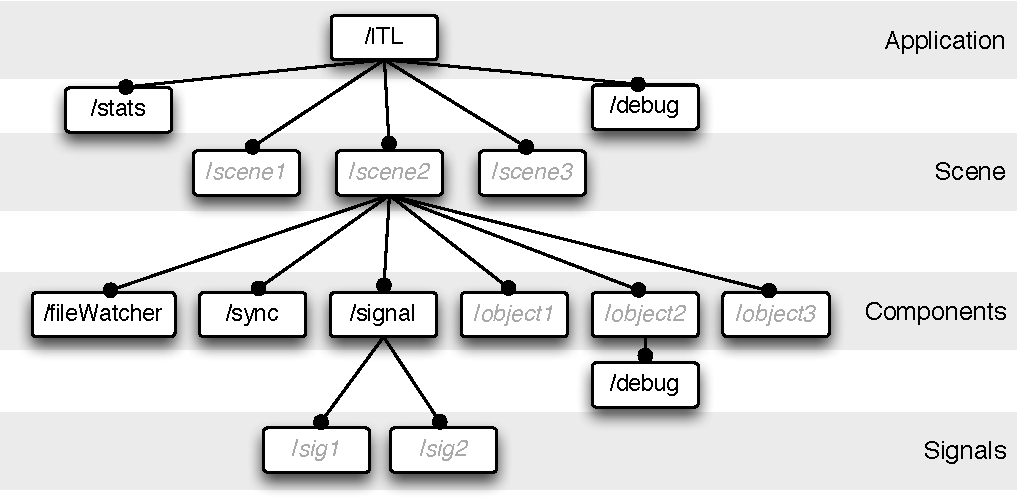
\includegraphics[width=120mm]{imgs/address_space}
 \caption{The OSC address space. Nodes in italic/blue are dynamic nodes.}
 \label{fig:addrspace}
\end{figure}

OSC messages are accepted at any level of the hierarchy:
\begin{itemize}
\item the application level responds to messages for application management (udp ports management, loading files, query messages). \\
It includes a static node named \OSC{stats} that collects statistics about incoming messages, and a static \OSC{debug} node that can be used to get debug information.
\item at \emph{scene} level, each node is associated to a window and respond to specific scene/window management messages.
\item the \emph{component} level contains the scene objects and two static nodes:

\begin{itemize}
\item a \emph{signal} node that may be viewed as a folder containing signals
\item a \emph{sync} node, in charge of the synchronization messages
\end{itemize}
Each component includes a status node named \OSC{debug} that provides debugging information.
\item the \emph{signals} level contains signals i.e. objects that accept data streams an d that may be graphically rendered as a scene component.

\end{itemize}


%===============================
\sublevel{Aliases}
\label{alias}
An alias mechanism allows an arbitrary OSC address to be used in place of a real address. An \OSC{alias} message is provided to describe aliases: 
\begin{rail}
alias : OSCAddress 'alias' (([1] OSCAlias (message | ) ) | [2])
\end{rail}
\index{Common messages!alias}
\begin{itemize}
\item \textbf{[1]} sets \OSC{OSCAlias} as an alias of \OSC{OSCAddress}. The alias may be optionally followed by a message string which is then taken as an implied message i.e. the alias is translated to \OSC{OSCAddress message}.
\item \textbf{[2]} removes \OSC{OSCAddress} aliases.
\end{itemize}

Example:
\sample{/ITL/scene/myobject alias '/1/fader1'}
makes the object \OSC{myobject} addressable using the address \OSC{/1/fader1}.

Note that regular expressions are not supported by the alias mechanism and could lead to unpredictable results.


%===============================
%:ITL messages
\toplevel{Application messages}
\label{ITL}
Application messages are accepted by the static OSC address \OSC{/ITL}. 


%===============================
%: Application management
\sublevel{Application management}

\begin{rail}
ITLMsg : 'quit' 
		| ('rootPath' path) 
		| ('mouse' ('show' | 'hide'))
		| ('defaultShow' int32)
		| ('load' filePath)
		| ('require' int32 oscMsg)
		| ('time' int32)
		| ('rate' int32)
		| 'hello'
\end{rail}
\index{ITL messages!rootPath}
\index{ITL messages!mouse}
\index{ITL messages!defaultShow}
\index{ITL messages!load}
\index{ITL messages!hello}
\index{ITL messages!require}
\index{ITL messages!rate}
\index{ITL messages!time}

\begin{itemize}
\item \OSC{quit}: requests the client application to quit.

\item \OSC{rootPath}: \emph{rootPath} of an Interlude application is the default path where the application reads or writes a file when a relative path is used for this file. The default value is the user home directory. Sending the \OSC{rootPath} message without parameter resets the application path to its default value.

\item \OSC{mouse}: hide or show the mouse pointer.

\item \OSC{defaultShow}: changes the default \OSC{show} status for new objects. \\
The default \OSC{defaultShow} value is 1.

\item \OSC{load}: loads a file previously saved using the \OSC{save} message (see section \fullref{common}). Note that the load operation appends the new objects to the existing scene. When necessary, it is the sender responsibility to clear the scene before loading a file.

\item \OSC{require}: check for a version number equal or greater to the number given as argument. The version number should be encoded as an integer value (for example: 76 for version 0.76, 112 for version 1.12). An OSC message is associated to the require message with the same syntax and semantic described in section \fullref{interaction}. This message is triggered when the check fails.

\item \OSC{rate}: changes the time task rate. Note that null values are ignored.\\
The default \OSC{rate} value is 10.

\item \OSC{time}: sets the application current time. The current rate is internally added to the current time by the time task.

\item \OSC{hello}: query the host IP number. The message is intended for ITL applications discovery. Answer to the query has the following format: \\
\oldexample \OSC{IP  inPort outPort errPort} where \OSC{IP} is sent as a string and port numbers as integer values.

\end{itemize}

\example \\
when sending the message:
\sample{/ITL hello}
the application will answer with the following message:
\sample{/ITL 192.168.0.5  7000 7001 7003}
when it runs on a host which IP number is \OSC{192.168.0.5} using the default port numbers.

%===============================
%: Ports management
\sublevel{Ports management}
\label{ITLPorts}

\begin{rail}
ITLPortsMsg : ('port' int32)
		| ('outport' int32)
		| ('errport' int32)
\end{rail}
\index{ITL messages!port}
\index{ITL messages!outport}
\index{ITL messages!errport}

Changes the UDP port numbers:
\begin{itemize}
\item \OSC{port} defines the listening port number, 
\item \OSC{outport} defines the port used to send replies to queries, 
\item \OSC{errport} defines the port used to send error messages. 
\end{itemize}
The \OSC{int32} parameter should be a positive value in the range \values{[1024-49150]}. \\
The default \OSC{port}, \OSC{outport} and \OSC{errport} values are 7000, 7001 and 7002.

Note that error messages are sent as a single string.

%===============================
%: Messages forwarding
\sublevel{Messages forwarding}
\label{ITLForward}

The messages handled by the application can be forwarded to arbitrary remote hosts using the \OSC{forward} message. The \OSC{forward} message itself can't be forwarded. 
 
\begin{rail}
ITLMsgForward : ('forward' ( [1] | [2] hostname +))
\end{rail}
\index{ITL messages!forward}

\begin{itemize}

\item 1) removes the set of forwarded destinations,
\item 2) set a list of remote hosts for forwarding. Note that \OSC{hostname} can be any legal host name or IP number, optionally extended with a port number separated by a semi-colon. By default, when no port number is specified, the current application listening port number is used.
\end{itemize}
\example
\sample{/ITL forward host1.adomain.org host2.adomain.org:5100}
Forwards messages to \OSC{host1.adomain.org} using the current application listening port number \\
and to \OSC{host2.adomain.org} on port number 5100.

\warning{forwarding messages to the application host results in an infinite loop with unpredictable results. Thus it is not recommended to use the local network broadcast address for forwarding.}



%===============================
%: Application level queries
\sublevel{Application level queries}
\label{ITLQuery}

The application supports the \OSC{get} messages for its parameters (see section \fullref{getsect}). In addition, it provides the following messages to query version numbers.

\begin{rail}
ITLRequest : 'get'  ('version' | 'guido-version' | 'musicxml-version')
\end{rail}
\index{ITL messages!version}
\index{ITL messages!guido-version}
\index{ITL messages!musicxml-version}

\begin{itemize}
\item \OSC{version}: version number request.
\item \OSC{guido-version}: Guido engine version number request.
\item \OSC{musicxml-version}: MusicXML and Guido converter version numbers request. Returns "not available" when the library is not found.

\end{itemize}



%===============================
%:Scene messages
\toplevel{Scene messages}
\label{scene}
A scene may be viewed as a window on the score elements. Its address is \OSC{/ITL/\textit{sceneIdentifier}} where \OSC{\textit{sceneIdentifier}} is the scene name. It handles the following messages:
\begin{rail}
sceneMsg :  'new'
			| 'del'
			| 'reset'
			| ('rootPath' path) 
			| ('load' filePath)
			| ('fullscreen' int32)
			| ('frameless' int32)
			| ('absolutexy' int32)
			| commonMsg
\end{rail}
\index{Scene messages}
\index{Scene messages!new}
\index{Scene messages!del}
\index{Scene messages!rootPath}
\index{Scene messages!load}
\index{Scene messages!reset}
\index{Scene messages!fullscreen}
\index{Scene messages!frameless}
\index{Scene messages!absolutexy}

\begin{itemize}
\item \OSC{new}: creates a new scene and opens it in a new window.
\item \OSC{del}: deletes a scene and closes the corresponding window.
\item \OSC{reset}: clears the scene (i.e. delete all components) and resets the scene to its default state (position, size and color).
\item \OSC{rootPath}: \emph{rootPath} of a scene is the default path where the scene reads or writes a file when a relative path is used for this file. When no value has been specified, the application  \emph{rootPath} is used.
\item \OSC{load}: loads an INScore file to the scene. Note that the OSC addresses are translated to the scene OSC address.
%\item \OSC{foreground}: put the scene to foreground.
\item \OSC{fullscreen}: requests the scene to switch to full screen or normal screen.  The parameter is interpreted as a boolean value. Default value is \values{0}.
\item \OSC{frameless}: requests the scene to switch to frameless or normal window.  The parameter is interpreted as a boolean value. Default value is \values{0}.
\item \OSC{absolutexy}: requests the scene to absolute or relative coordinates. Absolute coordinates are in pixels relative to the top left corner of the screen. Relative coordinates are in the range [-1, 1] where [0,0] is the center of the screen. The message parameter is interpreted as a boolean value. Default value is \values{0}.
\item \OSC{commonMsg}: see section \fullref{common}.
\end{itemize}


%===============================
%:Common messages
\toplevel{Common messages}
\label{common}
Common messages are mainly intended to control the graphic appearance of the components and  of the scene.
They could be sent to any address with the form \OSC{/ITL/scene} or \OSC{/ITL/scene/\textit{identifier}} where \OSC{\textit{identifier}} is the unique identifier string of a scene component.
\begin{rail}
commonMsg :  ('show' int32)
			| 'del'
			| 'export' ([1] ( fullPathFileName) | [2] path | [3])
			| 'save' filePath ( | '+')
			| PositionMsg
			| ColorMsg
			| TimeMsg
			| WatchMsg
\end{rail}
\index{Common messages!show}
\index{Common messages!del}
\index{Common messages!export}
\index{Common messages!save}

\begin{itemize}
\item \OSC{show}: shows or hides the destination object. The parameter is interpreted as a boolean value. Default value is \values{1}. 
\item \OSC{del}: deletes the destination object. 

\item \OSC{export}: exports an object to an image file. \\
1) exports to a full path name. The file extension is used to infer the export format. Supported extensions and formats are: \emph{pdf, bmp, gif, jpeg, png, pgm, ppm, tiff, xbm, xpm}. \\
2) exports to \OSC{path/\textit{identifier}.pdf}. When path is a relative path, exports to \OSC{rootPath/path/\textit{identifier}.pdf}. \\
3) exports to \OSC{rootPath/\textit{identifier}.pdf}.\\
When the destination file is not completely specified (third form or missing extension), there is an automatic numbering of output names when the destination file already exists.

\item \OSC{save}: recursively saves objects states to a file.  The \OSC{filePath} can be relative or absolute. When relative, an absolute path is build using the current \OSC{rootPath}. The optional \OSC{+} parameter indicates an append mode for the write operation. The message must be sent to the \OSC{/ITL} address to save the whole application state.\\
Note that the file extension for INScore files is \OSC{.inscore}. INScore files dropped on the application or on a window are interpreted as script files (see section \fullref{scripting}).

%\item \OSC{rename}: rename the destination object. Changes its OSC address. \textbf{Warning}: OSC pattern matching allows to give the same name to a whole collection of objects; in this case, there is no way to individually address an object when its name is shared with other objects.
\item 'PositionMsg' are absolute and relative position messages.
\item 'ColorMsg' are absolute and relative color control messages.
\item 'TimeMsg' are time management messages. They are described in section \fullref{time}.
\item 'WatchMsg' are described in section \fullref{interaction}.
%\item 'clickSelectMsg' are provided to query objects relative positions.
\end{itemize}

Examples:\\
Export of a scene to a given file as jpeg at the current root path:
\sample{/ITL/scene export 'myexport.jpg'}
Saving a scene to \OSC{myScore.inscore} at the current root path, the second form uses the append mode:
\sample{/ITL/scene save 'myScore.inscore'\\
/ITL/scene save 'myScore.inscore' '+'}

%-------------------------------
%:   Positioning
\sublevel{Positioning}

\begin{rail}
PositionMsg : 		absPosMsg 
				|	relPosMsg 
				|	originMsg 
				| 	transformMsg
\end{rail}

Graphic position messages are absolute position or relative position messages. They can also control an object \emph{origin} and transformations like rotation around an axis.

\subsublevel{Absolute positioning}

\begin{rail}
absPosMsg :  
			('x' float32)
		| 	('y' float32)
		| 	('z' float32)
		| 	('angle' float32)
		| 	('scale' float32) 
\end{rail}
\index{Position messages!absolute!x}
\index{Position messages!absolute!y}
\index{Position messages!absolute!z}
\index{Position messages!absolute!angle}
\index{Position messages!absolute!scale}
\index{Common messages!x}
\index{Common messages!y}
\index{Common messages!z}
\index{Common messages!angle}
\index{Common messages!scale}

\begin{itemize}
\item \OSC{x y}: moves the \values{x} or \values{y} coordinate of a component. By default, components are centered on their \values{x}, \values{y} coordinates. The coordinates space range is \values{[-1,1]}. \\
For a \OSC{scene} component, -1 is the leftmost or topmost position, 1 is the rightmost or bottommost position. \values{[0,0]} represents the center of the \OSC{scene}. \\
For the \OSC{scene} itself, it moves the window in the screen space and the coordinate space is orthonormal, based on the screen lowest dimension (\emph{i.e.} with a 4:3 screen, \OSC{y=-1} and \OSC{y=1} are respectively the exact top and bottom of the screen, but neither \OSC{x=-1} nor \OSC{x=1} are the exact left and right of the screen). \\
Default coordinates are \values{[0,0]}.
\item \OSC{z}: sets the \values{z} order of a component. The range is $[0,\infty[$. \values{z} order is actually relative to the \OSC{scene} components: objects of high \values{z} order will be drawn on top of components with a lower \values{z} order. Components sharing the same \values{z} order will be drawn in an undefined order, although the order will stay the same for as long as they live. \\
Default \values{z} order is 0.
\item \OSC{angle}: sets the \values{angle} value of a component, which is used to rotate it around its center. The angle is measured in clockwise degrees from the \values{x} axis.\\
Default angle value is 0.
\item \OSC{scale}: reduce/enlarge a component. The range is $[0,\infty[$. Default scale is \values{1}.
\end{itemize}

%-------------------------------
%:   Relative positioning
\subsublevel{Relative positioning}
\label{relpos}

\begin{rail}
relPosMsg :  
			('dx' float32)
		| 	('dy' float32)
		| 	('dz' float32)
		| 	('dangle' float32)
		| 	('dscale' float32) 
\end{rail}
\index{Position messages!relative!dx}
\index{Position messages!relative!dy}
\index{Position messages!relative!dz}
\index{Position messages!relative!dangle}
\index{Position messages!relative!dscale}
\index{Common messages!dx}
\index{Common messages!dy}
\index{Common messages!dz}

\begin{itemize}
\item \OSC{dx}, \OSC{dy}, \OSC{dz} messages are similar to \OSC{x}, \OSC{y}, \OSC{z} but the parameters represent a displacement relative to the current target value.
\item \OSC{dscale} is similar to \OSC{scale} but the parameters represents a scale multiplying factor.
\end{itemize}

%-------------------------------
%:   Components origin
\subsublevel{Components origin}
\label{origin}

The origin of a component is the point $(x_o, y_o)$ such that the $(x, y)$ coordinates and the $(x_o, y_o)$ point coincide graphically. For example, when the origin is the top left corner, the component top left corner is drawn  at the $(x, y)$ coordinates.

\begin{rail}
originMsg :  
			('xorigin' float32)
		| 	('yorigin' float32)
		| 	('dxorigin' float32)
		| 	('dyorigin' float32)
\end{rail}
\index{Position messages!relative!xorigin}
\index{Position messages!relative!yorigin}
\index{Position messages!relative!dxorigin}
\index{Position messages!relative!dyorigin}

\begin{itemize}
\item \OSC{xorigin}, \OSC{yorigin} are relative to the component coordinates space i.e. $[-1,1]$, where -1 is the top or left border and 1 is the bottom or right border. The default origin is $[0,0]$ i.e. the component is centered on its $(x,y)$ coordinates.
\item \OSC{dxorigin}, \OSC{dyorigin} represents displacement of the current \OSC{xorigin} or \OSC{yorigin}.
\end{itemize}


%-------------------------------
%:   Components transformations
\sublevel{Components transformations}
\label{transform}

A component tranformation specifies 2D transformations of its coordinate system. It includes shear and object rotation.

\begin{rail}
transformMsg :
			(('rotatex' | 'rotatey' | 'rotatez') float32)
		| 	('shear' x y)
\end{rail}
\index{Transform messages!rotate}
\index{Transform messages!shear}

\begin{itemize}
\item \OSC{rotatex rotatey rotatez}: rotates the component around the corresponding axis. Parameter value expresses the rotation in degrees.
\item \OSC{shear} transforms the component in x and y dimensions. \OSC{x} and \OSC{y} are float values expressing the transformation value in the corresponding dimension.
\end{itemize}

%-------------------------------
%:Color messages
\sublevel{Color messages}
\label{colormsg}


\begin{rail}
ColorMsg : 	absColorMsg 
			|	relColorMsg 
\end{rail}

Color messages are absolute or relative color control messages. Color may be expressed in RGBA or HSBA.

\subsublevel{Absolute color messages}

\begin{rail}
absColorMsg :    color
			| hsb
			| 'red' colorvalue
			| 'green' colorvalue
			| 'blue' colorvalue
			| 'alpha' colorvalue
			| 'hue' colorvalue
			| 'saturation' colorvalue
			| 'brightness' colorvalue
\end{rail}
\index{Common messages!color}
\index{Common messages!color!red}
\index{Common messages!color!blue}
\index{Common messages!color!green}
\index{Common messages!color!alpha}
\index{Common messages!color!hue}
\index{Common messages!color!saturation}
\index{Common messages!color!brightness}


\OSC{red}, \OSC{green}, \OSC{blue}, \OSC{hue}, \OSC{saturation}, \OSC{brightness}, \OSC{alpha} messages address a specific part of a color using RGB or HSB schemes.
The value may be specified as integer or float values. When expressed as float, the range is \values{[-1,1]}. The correspondence between the float and integer ranges is given below.

\begin{rail}
colorvalue :    int32 | float32
\end{rail}

\begin{rail}
color :		'color' ('r' 'g' 'b' | 'r' 'g' 'b' 'a') 
\end{rail}
\index{Common messages!color}

\OSC{color} sets an object color. The color scheme is RGBA. 
When A is not specified, the color is assumed to be opaque. 
The integer data range for each color component is \values{[0,255]}.
The float data range \values{[-1,1]} is linearly mapped to \values{[0,255]}. \\
Default color value is \values{[0,0,0,255]}.

\begin{rail}
hsb :		'hsb' ('h' 's' 'b' | 'h' 's' 'b' 'a') 
\end{rail}
\index{Common messages!hsb}

\OSC{hsb} is similar to \OSC{color} but using an HSBA scheme. 
When A is not specified, the color is assumed to be opaque. 
The data range for S, B is \values{[0,100]}, \values{[0,360]} for H, and \values{[0,255]} for A. \\
The float data range \values{[-1,1]} is mapped to \values{[0,100]} for S and B. 
For H, \values{0} refers always to the red color and thus \values{[0,1]} is mapped to \values{[0,180]} and \values{[-1,0]} is mapped to \values{[360,180]}.


%-------------------------------
%:   Relative color messages
\subsublevel{Relative color messages}
\label{relcolormsg}

\begin{rail}
relColorMsg :  
		 	('dcolor' color) 
		| 	('dhsb' hsb) 
		| 	('dred' colorvalue) 
		| 	('dgreen' colorvalue) 
		| 	('dblue' colorvalue) 
		| 	('dhue' colorvalue) 
		| 	('dsaturation' colorvalue) 
		| 	('dbrightness' colorvalue) 
		| 	('dalpha' colorvalue) 
\end{rail}
\index{Position messages!color!dcolor}
\index{Position messages!color!dhsb}
\index{Position messages!color!dred}
\index{Position messages!color!dgreen}
\index{Position messages!color!dblue}
\index{Position messages!color!dhue}
\index{Position messages!color!dsaturation}
\index{Position messages!color!dbrightness}
\index{Position messages!color!dalpha}

\begin{itemize}
\item \OSC{dred}, \OSC{dgreen}, etc. messages are similar to \OSC{red}, \OSC{green}, etc. messages but the parameters values represent a displacement of the current target value.
\item \OSC{dcolor} and \OSC{dhsb} are similar and each color parameter represents a displacement of the corresponding target value.
\end{itemize}


%-------------------------------
%:'effect' messages
\sublevel{The 'effect' messages}
\label{effectmsg}

The \OSC{effect} message sets a graphic effect on the target object.

\begin{rail}
effectMsg : 'effect' ( 'none'
		| ('blur'
		| 'colorize'
		| 'shadow') (| params)) 		
\end{rail}
\index{Effect messages!effect!none}
\index{Effect messages!effect!blur}
\index{Effect messages!effect!colorize}
\index{Effect messages!effect!shadow}

\begin{itemize}
\item \OSC{none}: removes any effect set on the target object.
\item \OSC{blur, colorize, shadow}: sets the corresponding effect. An effect always replaces any previous effect. The effect name is followed by optional specific effects parameters.
\end{itemize}

Note that an effect affects the target object but also all the target slaves.

\subsublevel{The blur effect}

\begin{rail}
blurParams : int32 (| blurHint)
\end{rail}

Blur parameters are the blur radius and a rendering hint. The radius is an int32 value. By default, it is 5 pixels. The radius is given in device coordinates, meaning it is unaffected by scale. 

\begin{rail}
blurHint : 'performance' | 'quality' | 'animation'
\end{rail}
Use the \OSC{performance} hint to say that you want a faster blur, the \OSC{quality} hint to say that you prefer a higher quality blur, or the \OSC{animation} when you want to animate the blur radius. The default hint value is \OSC{performance}.

\subsublevel{The colorize effect}

\begin{rail}
colorizeParams : float32 (| color)
\end{rail}

Colorize parameters are a strength and a tint color. The strength is a float value. By default, it is 1.0. A strength 0.0 equals to no effect, while 1.0 means full colorization. \\
The color is given as a RGB triplet (see \fullref{colormsg}) by default, the color value is light blue (0, 0, 192).


\subsublevel{The shadow effect}

\begin{rail}
shadowParams : xoffset yoffset (| color (| blur))
\end{rail}

\OSC{xoffset} and \OSC{yoffset} are the shadow offset and should be given as int32 values. The default value is 8 pixels. The offset is given in device coordinates, which means it is unaffected by scale. \\
The color is given as a RGBA color (see \fullref{colormsg}) by default, the color value is a semi-transparent dark gray (63, 63, 63, 180) \\
The blur radius should be given as an int32 value. By default, the blur radius is 1 pixel.

%-------------------------------
%:The 'click' and 'select' messages
%\sublevel{The 'click' and 'select' messages}
%\label{csmsg}
%
%\textbf{Warning}: the \OSC{click} and \OSC{select} messages are deprecated and will be removed in a future version.
%
%The \OSC{click} and \OSC{select} messages can be sent to any address with the form \OSC{/ITL/scene/\textit{identifier}} where \OSC{\textit{identifier}} is the unique identifier string of a scene component. They are intended to provide information about components relative positions: it returns a list of components identifiers that are 'under' the \emph{clicked} component: z order of the components is used for the 'under' relationship. 
% 
%\begin{rail}
%click :		'click' ( | clickMode)
%\end{rail}
%\index{Common messages!click}
% 
%\begin{rail}
%clickMode :	'topleft' | 'bottomright' | 'topright' | 'bottomleft' | 'center'
%\end{rail}
%\index{Common messages!click!topleft}
%\index{Common messages!click!bottomright}
%\index{Common messages!click!topright}
%\index{Common messages!click!bottomleft}
%\index{Common messages!click!center}
%
% 
%\begin{itemize}
%\item \OSC{topleft}, \OSC{bottomright}, \OSC{topright}, \OSC{bottomleft}, \OSC{center}: collects the components that are respectively under the top-left, bottom-right, top-right, bottom-left or center point of the target component. The clicked point is computed from the component bounding box.
%\item Sent without parameter, the \OSC{click} message is equivalent to \OSC{click topleft}.
%\end{itemize}
%
%Reply of the \OSC{click} message has the following form:
%\begin{rail}
%clickReply :	OSCAddress	clickMode ( | (identifier +))
%\end{rail}
%
%where 'identifier' is a component name. Note that 'identifiers' are sorted by decreasing z order.
%
%\begin{rail}
%select :	'select' ( 	| selectMode)
%\end{rail}
%\index{Common messages!select}
% 
%\begin{rail}
%selectMode :	'intersect' | 'include'
%\end{rail}
%\index{Common messages!select!intersect}
%\index{Common messages!select!include}
%
%\begin{itemize}
%\item \OSC{intersect}: looks for the components that are under the \emph{clicked} component and that intersect with its bounding box.
%\item \OSC{include}: looks for the components that are under the \emph{clicked} component and that are included in its bounding box.
%\item Sent without parameter, the \OSC{select} message is equivalent to \OSC{select intersect}.
%\end{itemize}
%
%Reply of the \OSC{select} message is similar to \OSC{click} reply:
%\begin{rail}
%selectReply :	OSCAddress	selectMode ( | (identifier +))
%\end{rail}


%===============================
%:Time management messages
\toplevel{Time management messages}
\label{time}
Time messages control the time dimension of the score components. They could be sent to any address with the form \OSC{/ITL/scene/\textit{identifier}} where \OSC{\textit{identifier}} is the unique identifier string of a scene component.
\begin{rail}
timeMsg : 'clock'
		| 'durClock' 
		| ('date' time)
		| ('duration' time) 
		| ('ddate' time) 
		| ('dduration' time) 
\end{rail}
\index{Time messages!absolute!date}
\index{Time messages!absolute!duration}
\index{Time messages!relative!ddate}
\index{Time messages!relative!dduration}
\index{Time messages!relative!clock}
\index{Time messages!relative!durClock}

\begin{rail}
time : (([1] int32 int32) | [2] int32 | [3] float32 | [4] 'n/d')
\end{rail}

\begin{itemize}
\item 1) Time is specified as a rational value \values{d/n} where \values{1/1} represents a whole note. 
\item 2) Time may be specified with a single integer, then 1 is used as implicit denominator value
\item 3) Time may be specified as a single float value that is converted using the following approximation: let \values{f} be the floating point date, the corresponding rational date is computed as \values{f x 10000 / 10000}.
\item 4) Time may also be specified as a string in the form \OSC{'n/d'}.
\end{itemize}

\begin{itemize}
\item \OSC{clock}: similar to MIDI clock message: advances the object date by 1/24 of quarter note.
\item \OSC{durClock}: a clock message applied to duration: increases the object duration by 1/24 of quarter note.
\item \OSC{date}: sets the time position of an object. Default value is \values{0/1}.
\item \OSC{duration}: changes the object duration. Default value is \values{1/1}.
\item \OSC{ddate}: relative time positioning message: adds the specified value to the object date.
\item \OSC{dduration}: relative duration message: adds the specified value to the object duration.
\end{itemize}


%===============================
%:The 'set' message
\toplevel{The 'set' message}
\label{setsect}
The \OSC{set} messages can be sent to any address with the form \OSC{/ITL/scene/\textit{identifier}}. The global form of the message is:

\begin{rail}
setMsg : 'set' type data
\end{rail}

It sets a \OSC{scene} component data. When there is no destination for the OSC address, the component is first created before being given the message. When the target destination type doesn't correspond to the message \OSC{type}, the object is replaced by an adequate object.


%===============================
%: Inline components
\sublevel{Inline components}
\label{inlineset}

Supported types are the following:
\begin{itemize}
\item \OSC{txt}: a textual component.
\item \OSC{html}: an html component defined by an HTML string.
\item \OSC{gmn}: a Guido score defined by a GMN string.
\item \OSC{svg}: SVG graphics defined by a SVG string.
\item \OSC{graph}: graphic of a signal. See section \fullref{graphsig} for details about the \OSC{graph} objects data.
\item \OSC{fastgraph}: fast rendering graphic signal. See also section \fullref{graphsig}.
\item \OSC{rect}: a rectangle specified by a width and height. Width and height are expressed in \OSC{scene} coordinates space, thus a width or a height of 2 corresponds to the width or a height of the \OSC{scene}.
\item \OSC{ellipse}: an ellipse specified by a width and height.
\item \OSC{polygon}: a polygon specified by a sequence of points, each point being defined by its (x,y) coordinates. The coordinates are expressed in the \OSC{scene} coordinate space, but only the relative position of the points is taken into account (\emph{i.e} a polygon A = \{ (0,0) ; (1,1) ; (0,1) \} is equivalent to a polygon B = \{ (1,1) ; (2,2) ; (1,2) \}).
\item \OSC{curve}: a sequence of 4-points bezier cubic curve. If the end-point of a curve doesn't match the start-point of the following one, the curves are linked by a straight line. The first curve follows the last curve. The inner space defined by the sequence of curves is filled, using the object color. The points coordinates are handled like in a \OSC{polygon}.
\item \OSC{line}: a simple line specified by a point (x,y) expressed in \OSC{scene} coordinate space or by a width and angle. The point form is used to compute a line from (0,0) to (x,y), which is next drawn centered on the scene.
\end{itemize}

Format of the \OSC{set} message is:
\begin{rail}
setMsg : 'set' (
	('txt' txtStream) |
	('html' string) |
	('svg' svgString) |
	('gmn' gmnString) |
	('graph' signals ) |
	('fastgraph' signals ) |
	('rect' width height) |
	('ellipse' width height) |
	('polygon' ( (x y) +)) |
	('curve' ((x1 y1 x2 y2 x3 y3 x4 y4) +)) |
	('line' ('xy' x y | 'wa' width angle)) |
	setFile
)
\end{rail}
\index{Common messages!set}
\index{Set type!txt}
\index{Set type!html}
\index{Set type!svg}
\index{Set type!gmn}
\index{Set type!graph}
\index{Set type!rect}
\index{Set type!ellipse}
\index{Set type!polygon}
\index{Set type!curve}
\index{Set type!line}

Note that the default position of any component is \values{[0,0]}. Objects are drawn centered on their position.

\begin{rail}
txtStream :  (string | int32 | float32) +
\end{rail}


%===============================
%: File based components
\sublevel{File based components}
\label{fileset}


\label{setfile}
\begin{rail}
setFile : 
	('txtf' textFilePath) |
	('htmlf' htmlFilePath) |
	('gmnf' gmnFilePath) |
	('svgf' svgFilePath) |
	('img' imgPath) |
	('video' videoPath) |
	('file' filePath)
\end{rail}
\index{Set type!txtf}
\index{Set type!htmlf}
\index{Set type!gmnf}
\index{Set type!img}
\index{Set type!video}
\index{Set type!svg}
\index{Set type!file}

\begin{itemize}
\item \OSC{txtf}: a textual component defined by a file.
\item \OSC{htmlf}: an html component defined by an HTML file.
\item \OSC{gmnf}: a Guido score defined by a GMN file.
\item \OSC{svgf}: vectorial graphics defined by a SVG file.
\item \OSC{img}: an image file based component. The image format is infered from the file extension.
\item \OSC{video}: a video file based component. The video format is infered from the file extension. Note that navigation through the video is made using its \OSC{date}.
\item \OSC{file}: a generic type to handle file based objects. Actually, the \OSC{file} type is translated into a one of the \OSC{txtf}, \OSC{gmnf}, \OSC{img} or \OSC{video} types, according to the file extension (see table \ref{fileTranslate}).
\end{itemize}

\seealso the application \OSC{rootPath} message (section \ref{ITL}) for file based objects.

\begin{table}[htdp]
\caption{File extensions supported by the \OSC{file} translation scheme.}
\begin{center}
\begin{tabular}{|r|c|}
\hline
file extension & translated type \\
\hline
\OSC{.txt .text}		& \OSC{txtf} \\
\OSC{.htm .html}		& \OSC{htmlf} \\
\OSC{.gmn .xml}		& \OSC{gmnf} \\
\OSC{.svg} 			& \OSC{svgf} \\
\OSC{.jpg .jpeg .png .gif .bmp .tiff} & \OSC{img} \\
\OSC{.avi .wmv .mpg .mpeg .mp4} & \OSC{video} \\
\hline
\end{tabular}
\end{center}
\label{fileTranslate}
\end{table}


%===============================
%:The 'get' message
\toplevel{The 'get' messages}
\label{getsect}

%-------------------------------
%\sublevel{Common 'get' format}
The \OSC{get} messages can be sent to any valid OSC address. It is intended to query the system state. It is the counterpart of all the messages modifying this state.  The result of the query is sent to the OSC output port with the exact syntax of the counterpart message. 
The global form of the message is:
\begin{rail}
getMsg : 'get' ( | getParam +)
\end{rail}
\index{Common messages!get}

The \OSC{get} message without parameter is the counterpart of the \OSC{set} message. 

\example \\
Sending the following request to an object which position is 0.3 0.5
\sample{/ITL/scene/myobject get x y}
will give the following messages on outpout port:
\sample{/ITL/scene/myobject x 0.3 \\
/ITL/scene/myobject y 0.5}

%-------------------------------
\sublevel{Special 'get' forms}

The \OSC{get} message without parameter addressed to a container (the application \OSC{/ITL}, a scene \OSC{/ITL/scene}, the signal node \OSC{/ITL/scene/signal}) is also distributed to all the container components.


The \OSC{get width} and \OSC{get height} messages adressed to components that have no explicit width and height (text, images, etc.) return 0 as long as the target component has not been drew.



%===============================
%:Component specific messages
\toplevel{Component specific messages}
\label{specificMsg}
Some of the messages are specific to the component \OSC{type}. These messages can be sent to addresses of the form \OSC{/ITL/scene/\textit{identifier}}. They are ignored by objects that don't support the message. 

%-------------------------------
\sublevel{Pen control}

Messages accepted by the components types \OSC{rect | ellipse | polygon | curve | line | graph}.
\begin{rail}
penMsg : 	  'penColor' color 
			| 'penWidth' float32
			| 'penStyle' penstyle
\end{rail}
\index{Specific messages! penColor}
\index{Specific messages! penWidth}
\index{Specific messages! penStyle}

\begin{rail}
penstyle : 'solid' | 'dash' | 'dot' | 'dashDot' | 'dashDotDot'
\end{rail}
\index{Specific messages! penStyle! solid}
\index{Specific messages! penStyle! dash}
\index{Specific messages! penStyle! dot}
\index{Specific messages! penStyle! dashDot}
\index{Specific messages! penStyle! dashDotDot}

The pen width default value is 0 (excepted for \OSC{line} objects, where 1.0 is the default value). It is expressed in arbitrary units (1 is a reasonable value).
The pen style default value is \OSC{solid}.\\
The color scheme is described in section \ref{colormsg}.


%-------------------------------
\sublevel{Width and height control}

Messages accepted by the components types \OSC{rect | ellipse | graph.}

\begin{rail}
whMsg : 	  'width' float32
			| 'height' float32
\end{rail}
\index{Specific messages! width}
\index{Specific messages! height}



%-------------------------------
\sublevel{Score pages management}
\label{gmnpage}

Messages accepted by the components types \OSC{gmn | gmnf}. 
\begin{rail}
scoreMsg :      'page' int32
			| 'dpage' int32
			| 'pageFormat' float32 float32
			| 'columns' int32
			| 'rows' int32
			| 'get' 'pageCount'
\end{rail}
\index{Specific messages! score! page}
\index{Specific messages! score! dpage}
\index{Specific messages! score! pageFormat}
\index{Specific messages! score! columns}
\index{Specific messages! score! rows}
\index{Specific messages! score! pageCount}


\begin{itemize}
\item \OSC{page}: set the score current page
\item \OSC{dpage}: set the score current page
\item \OSC{pageFormat}: set the page format. The parameters are the page width and height. Note that the message has no effect when the score already includes a $\backslash$pageformat tag.
\item \OSC{columns}: for multi pages display: set the number of columns.
\item \OSC{rows}: for multi pages display: set the number of rows.
\item \OSC{pageCount}:  a read only attribute, gives the score pages count.
\end{itemize}


%-------------------------------
%\sublevel{Video maps}
%
%Messages accepted by \OSC{video} components.
%\begin{rail}
%specificMsg : 	 'videoMap' ( 
%								( floatSegment relativeTimeSegment ) + 
%							| 	( ( 'tempo' float32 | ) ( 'startSecond' float32 | )  )
%							)
%				| 'videoMapf' string
%\end{rail}



%\begin{rail}
%specificMsg : 	  [5] 'curveType' curveType
%				| [5] 'thickness' thickness
%				| [5] 'drawLine' drawLine
%				| [5] 'ignoreSignalColor' int32
%				| [5] 'penIgnoreSignalColor' int32
%\end{rail}


%\begin{rail}
%curveType : 'round' | 'step'
%\end{rail}
%
%\begin{rail}
%thickness : 'centered' | 'up' | 'down'
%\end{rail}
%
%\begin{rail}
%drawLine : 'top' | 'bottom' | 'both'
%\end{rail}

%\index{Specific messages! ignoreSignalColor}
%\index{Specific messages! penIgnoreSignalColor}
%\index{Specific messages! curveType! round}
%\index{Specific messages! curveType! step}
%\index{Specific messages! thickness! centered}
%\index{Specific messages! thickness! up}
%\index{Specific messages! thickness! down}
%\index{Specific messages! drawLine! top}
%\index{Specific messages! drawLine! bottom}
%\index{Specific messages! drawLine! both}

%Graph specific messages:
%\begin{itemize}
%\item \OSC{curveType}: defines if the graph's shape should be smooth (\OSC{round}) or with steps, like in an histogram (\OSC{step}). Default: \OSC{round}.
%\item \OSC{thickness}: defines if the thickness of the graph's shape, starting from the 'y' value, should go \OSC{up}, \OSC{down}, or sould be \OSC{centered}. Default: \OSC{centered}.
%\item \OSC{drawLine}: defines if the top and bottom bounds of the graph's shape should be outlined using the graph's \OSC{penStyle} and \OSC{penWidth}. Note that if you don't want any outlining, just set the \OSC{penWidth} to 0. Default: \OSC{both}.
%\item \OSC{ignoreSignalColor}: If set, the color signal of the graph signal will be ignored, and the object's \OSC{color} will be used instead to fill the graph's shape. Default: 0.
%\item \OSC{penIgnoreSignalColor}: Same as \OSC{ignoreSignalColor}, but for the outlining of the graph's shape (use/don't use the \OSC{penColor}). Default: 0.
%\end{itemize}

%The \OSC{videoMap} specifies the relative time mapping of the \OSC{video}: it maps chronometric time segments (\OSC{floatSegment}) of the video, expressed in seconds, to relative time segments, so that it's possible to navigate through the video using its \OSC{date}.\\
%The \OSC{videoMap} can also be expressed by a \OSC{tempo} and a \OSC{startSecond}, thus defining an affine relation between relative time and chronometric time.\\
%When no \OSC{videoMap} has been specified, \OSC{video} components use a default \OSC{tempo=60.0} and a default \OSC{startSecond=0.0}.
%The \OSC{videoMapf} message is similar to the \OSC{videoMap} message but expects the path name of a file containing the mapping data.

%===============================
%:Time to space mapping
\toplevel{Time to space mapping}
\label{mapping}

Time to space mapping refers to the description of relationship between an object local graphic space and its time space. 

%===============================
%:   The 'map' message
\sublevel{The 'map' message}
\label{mapMsg}

The \OSC{map} messages can be sent to any address with the form \OSC{/ITL/scene/\textit{identifier}}. It is intended to describe the target object relation to time and sets a relation between an object segmentation and a time segmentation. 
The global form of the message is:

\begin{rail}
mapMsg : 'map' ( | mapName ) (relation	|	( del ))
\end{rail}
\index{Common messages!map}

\begin{rail}
relation : 
		([1] float2DSegment relativeTimeSegment ) +
	| 	([2] int2DSegment relativeTimeSegment ) +
	| 	([3] int1DSegment relativeTimeSegment ) + 
\end{rail}

Segments are expressed as a list of intervals. For a 1 dimension resource, a segment is a made of a single interval. For a 2 dimensions resource, a segment is a made of 2 intervals: an interval on the $x$-axis and one on the $y$-axis for graphic based resource, or an interval on columns and one on lines for text based resources. Intervals are right-opened.

The different kind of relations corresponds to:
\begin{itemize}
\item \textbf{[1]} a relation between a 2 dimensions segmentation expressed in float values and a relative time segmentation. These segmentations are used by \OSC{rect, ellipse, polygon, curve, line} components.
\item \textbf{[2]} a relation between a 2 dimensions segmentation expressed in integer values and a relative time segmentation. These segmentations are used by \OSC{txt, txtf, img} components. 
\item \textbf{[3]} a relation between a 1 dimension segmentation expressed in integer values and a relative time segmentation. These segmentations are used by the \OSC{graph} component and express a relation between a signal space and time.
\end{itemize}
Table \ref{maptable} summarizes the specific segmentations used by each component type. 

The specified \OSC{map} can be named with an optional \OSC{mapName} string; this name can be further reused, during object synchronization, to specify the mapping to use. When \OSC{mapName} is not specified, the mapping has a default \emph{empty name}.

The \OSC{del} command deletes the mapping specified with \OSC{mapName}, or the \emph{'empty name'} mapping if no map name is specified.


\begin{table}[htdp]
\caption{Mapping resources for each component}
\begin{center}
\begin{tabular}{|r|l|}
\hline
component type & segmentation type \\
\hline
\OSC{txt, txtf}		& int2DSegments \\
\OSC{img}			& int2DSegments \\
%\OSC{rect, ellipse, polygon, curve, line, video}	&  \textbf{vectorial2relativeTime} \\
\OSC{rect, ellipse, polygon, curve}	&  float2DSegments \\
\OSC{graph}			&  int1DSegments \\
\hline
\end{tabular}
\end{center}
\label{maptable}
\end{table}

Note for \OSC{html, htmlf} + guido score mappings


\begin{rail}
relativeTimeSegment : '(' relativeTimeInterval ')' 
\end{rail}
\begin{rail}
float2DSegment : '(' floatInterval floatInterval ')' 
\end{rail}
\begin{rail}
int2DSegment : '(' intInterval intInterval ')' 
\end{rail}
\begin{rail}
int1DSegment : '(' intInterval ')' 
\end{rail}


\begin{rail}
relativeTimeInterval : '[' rational ',' rational '[' 
\end{rail}
\begin{rail}
floatInterval : '[' float32 ',' float32 '['
\end{rail}
\begin{rail}
intInterval : '[' int32 ',' int32 '['
\end{rail}

Relative time is expressed as \OSC{rational} values where $1$ represents a whole note.

\begin{rail}
rational : int32 '/' int32
\end{rail}


%===============================
%:   The 'map+' message
\sublevel{The 'map+' message}
\label{mapAddMsg}
The \OSC{map+} messages is similar to the \OSC{map} message but doesn't replace the existing mapping data: the specified relations are added to the existing one.

\begin{rail}
mapAddMsg : 'map+' ( | mapName ) relation
\end{rail}
\index{Common messages!map+}


%===============================
%:   Mapping files
\sublevel{Mapping files}
\label{mapFileMsg}
The \OSC{mapf} messages is similar to the \OSC{map} message but gives the path name of a file containing the mapping data, along with the optional map name.
\begin{rail}
mapfMsg : 'mapf' ( | mapName ) mapFilePath
\end{rail}
\index{Common messages!mapf}



%-------------------------------
%:Synchronization
\toplevel{Synchronization}
\label{syncmsg}

Synchronization between components is achieved at \OSC{scene} level: a \OSC{sync} node is automatically embedded in the scene, its address is \OSC{/ITL/scene/sync} and it supports messages to add or remove a master / slave relation between components or to query the synchronizations state.
\begin{rail}
sync : syncIdentifier 
	 ( [1] syncIdentifier (| syncmode +) 
	   | [2])
	   | [3] 'get' ( | identifier)
\end{rail}
\index{Synchronization}
\index{Synchronization!get}


\begin{itemize}
\item \textbf{[1]} this is the \OSC{slave} \OSC{master} form followed by an optional synchronization mode. It adds a slave / master relation between components identified by identifier1 and identifier2. \\
\item \textbf{[2]} this is the \OSC{slave} form that removes the slave synchronization for the component identified by identifier1.
\item \textbf{[3]} the \OSC{get} message is intended to query the synchronization state. The optional parameter is the identifier of a component,
\end{itemize}
Synchronization between components has no effect if any of the required mapping is missing (see table \ref{maptable}).

\begin{rail}
syncIdentifier : [1] identifier 
		| [2] identifier ':' mapName
\end{rail}
\index{Synchronization! syncIdentifier}

Synchronization identifiers indicates 1) the name of a \OSC{scene} component or 2) the name of a \OSC{scene} component associated to a mapping name.


Note that the \OSC{sync} node doesn't responds to common component messages, but accept the \OSC{get} message. 
The \OSC{get} message without parameter is equivalent to a \OSC{get} message addressed to each object declared in the \OSC{sync} node.

%-------------------------------
%:   Synchronization modes
\sublevel{Synchronization modes}

Synchronizing a component \values{A} to a component \values{B} has the following effect:
\begin{itemize}
\item \values{A} position (x,y) is modified to match the \values{B} time position corresponding to \values{A} date.
\item depending on the optional \OSC{syncStretch}, \values{A} width and/or height are modified to match the  corresponding \values{B} dimensions (see below).
\item if \values{A} date has no graphic correspondance in \values{B} mapping (the date is not mapped, or out of \values{B} mapping bounds ), \values{A} won't be visible.
\end{itemize}

\begin{rail}
syncmode : syncHow| syncStretch | syncPos | mapName
\end{rail}
\index{Synchronization!syncmode}

\begin{rail}
syncHow : 'relative' | 'absolute'
\end{rail}
\index{Synchronization!syncHow}
\index{Synchronization!syncHow!relative}
\index{Synchronization!syncHow!absolute}

The synchronization mode makes use of the master time to graphic mapping to compute the slave position. It may also use the master current date, depending on the following options:
\begin{itemize}
\item \OSC{absolute}: the time position where the slave appears corresponds to the mapping absolute date only.
\item \OSC{relative}: the time position where the slave appears is relative to the mapping and the master current date.
\end{itemize}
By default, the relative mode is used.

\begin{rail}
syncStretch : 'h' | 'v' | 'hv'
\end{rail}
\index{Synchronization!syncStretch}
\index{Synchronization!syncStretch!h}
\index{Synchronization!syncStretch!v}
\index{Synchronization!syncStretch!hv}

The synchronization stretch mode has the following effect on the slave dimensions:
\begin{itemize}
\item \OSC{h}: the slave is horizontally stretched to align its begin and end dates to the corresponding master locations.
\item \OSC{v}: the slave is vertically stretched to the master vertical dimension.
\item \OSC{hv}: combines the above parameters.
\end{itemize}
By default, no stretching is applied.

\begin{rail}
syncPos : 'syncOver' | 'syncTop' | 'syncBottom'
\end{rail}
\index{Synchronization!syncPos}
\index{Synchronization!syncPos!syncOver}
\index{Synchronization!syncPos!syncTop}
\index{Synchronization!syncPos!syncBottom}

The synchronization position mode has the following effects on the slave \values{y} position:
\begin{itemize}
\item \OSC{syncOver}: the center of the slave is aligned to the master center.
\item \OSC{syncTop}: the bottom of the slave is aligned to the top of the master.
\item \OSC{syncBottom}: the top of the slave is aligned to the bottom of the master.
\end{itemize}
\index{Synchronization!syncPos!syncOver}
\index{Synchronization!syncPos!syncTop}
\index{Synchronization!syncPos!syncBottom}
The default synchronization mode is \OSC{syncOver}.

The optional 'mapName' string argument specifies which mapping of the master object should be used (see \OSC{map} message). If the master doesn't have a mapping with the specified 'mapName', the slave object won't be visible.
Not specifying the map name is equivalent to an \emph{empty name} mapping.


%===============================
%:Score specific messages
\toplevel{Score specific messages}

%-------------------------------
%:   Specific score mappings
\sublevel{Specific score mappings}
\label{guidomaps}

Music score mappings are automatically computed  by the system. However, since a score may support a large number of mappings (staff based, system based, voice based, etc.), music scores supports a specific \OSC{map} message to request the computation of a specific mapping. This message has the form:
\begin{rail}
scoreMapMsg : 'map' ('page' | 'system' | 'systemflat' | ('staff' 'staffNum') | 'voice' 'voiceNum' )
\end{rail}
\index{Synchronization!Guido map}
\index{Synchronization!Guido map!page}
\index{Synchronization!Guido map!system}
\index{Synchronization!Guido map!systemflat}
\index{Synchronization!Guido map!staff}
\index{Synchronization!Guido map!voice}

The Guido map name must be concatenated as a string (as a usual map name).

\begin{itemize}
\item \OSC{page}: a page level mapping
\item \OSC{system}: a system level mapping
\item \OSC{systemflat}: a system level mapping without system subdivision (one graphic segment per system)
\item \OSC{staff}: a staff level mapping: the staff indicated by the next parameter (between 1 and the score staves count).
\item \OSC{voice}: a voice level mapping: the voice indicated by the next parameter (between 1 and the score voices count).
\end{itemize}


The default synchronization mode for a Guido score is \OSC{staff1}.
Note that a voice may be distributed on several staves and thus a staff may contain serveral voices.


%-------------------------------
%:   Score browsing and layout
\sublevel{Score browsing and layout}
\label{guidolayout}

\begin{rail}
scoreMsg : 	  'page' int32
				| 'pageFormat' float32 float32
				| 'columns' int32
				| 'rows' int32
\end{rail}

\begin{itemize}
\item \OSC{page}: sets the first displayed page. Index starts at \values{1}. Default: \values{1}.

\item \OSC{pageFormat}: sets the score's page format, in cm (Warning: the \OSC{pageFormat} is not used when another page format is 'hard-coded' in the score's Guido code). Default: \values{(21.0 , 29.7)}.

\item \OSC{columns}: as multiples pages can be displayed and organized in a \emph{grid of pages}, \OSC{columns} sets the number of columns in the grid. Default: \values{2}.

\item \OSC{rows}: as multiples pages can be displayed and organized in a \emph{grid of pages}, \OSC{rows} sets the number of rows in the grid. Default: \values{1}.
\end{itemize}

%-------------------------------
%:   Score queries
\sublevel{Score queries}
\label{guidoqueries}

\begin{rail}
scoreQuery : 	'get' (
				'pageCount'
			| 	'pageDate' int32
			)
\end{rail}

\begin{itemize}
\item \OSC{pageCount}: gives the score page count.
\item \OSC{pageDate}: gives the time location of a page, which number is given as argument. The system reply has the form \OSC{pageDate pageNum date} where \OSC{pageNum} is the request page number given as argument and \OSC{date} is the page time location expressed as a ra	tional number.
\end{itemize}

Note that a score object duration is automatically set to the score duration. It can be retrieved using a \OSC{get duration} message.


%===============================
%:Virtual address space
\toplevel{Virtual address space}

Virtual address space extends the OSC address scheme to objects automatically embedded into other objects. 

%===============================
%:   File watcher
\sublevel{File watcher}
\label{watch}

The \OSC{fileWatcher} is a component automatically embedded at scene level. \\
It receives messages at the address \OSC{/ITL/scene/fileWatcher}.

The \OSC{fileWatcher} service monitors files on demand; it is aware of file modifications and file removals (or renamings, which is equivalent). The \OSC{fileWatcher} works with associations between a file and an OSC message : when a file change occurs, the file watcher posts the associated OSC message.

The \OSC{fileWatcher} is controlled with 4 messages:
\begin{itemize}
\item the \OSC{add} message is used to add a new 'file' - 'OSC message' association ;
\item the \OSC{remove} message is used to remove a 'file' - 'OSC message' association.
\item the \OSC{clear} message is used to clear all existing associations.
\item the \OSC{get} message is used to retrieve the current associations.
\end{itemize}
\index{fileWatcher}

\begin{rail}
fileWatcher : ('add' filePath OSCMessage) 
		| 'remove' (filePath OSCMessage | OSCAddress )
		| 'clear'
		| 'get'
\end{rail}
\index{fileWatcher!add}
\index{fileWatcher!remove}
\index{fileWatcher!clear}
\index{fileWatcher!get}

where \OSC{OSCMessage} is any message complying to the format desscribed in section \fullref{genformat}.

\example
\sample{
/ITL/scene/fileWatcher add 'fuga.gmn' '/ITL/scene/score' 'set' 'gmnf' 'fuga.gmn';
}

Note that the \OSC{get} query returns a set of messages complying to the \OSC{add} message format.\\

The \OSC{remove} message may take only 1 parameter, in which case the only parameter is an OSC address : it stops monitoring any file associated to an OSC message with this OSC address.

Note that an OSC message can be associated to several files, and that a file can be associated to several OSC messages.
When a file has been removed (or renamed), the \OSC{fileWatcher} stops monitoring it.

\sublevel{Debug}

Each object has a \OSC{debug} sub-node for debugging purposes. This \OSC{debug} virtual node has 3 flags, that can be actived or desactived with \OSC{0} or \OSC{1}:

\begin{rail}
debug : 		('name'  int32)
		|	('map' int32)
		|	('signal' int32)
\end{rail}

\begin{itemize}
\item When the \OSC{name} flag is on, each scene component displays its bounding rectangle and name.
\item When the \OSC{map} flag is on, each scene component displays its mappings.
\item When the \OSC{signal} flag is on, each object (even the scene or the application) will, according to its type, emit 'performance related' signals (or no signal). This 'performance signal' is specific to the type of object. The name of 'performance signal' is of the form \OSC{debug-}\emph{objectName}\OSC{-}\emph{SomeName}. Currently, only the \OSC{application}, the \OSC{scene} and \OSC{graph} objects emit 'performance signals'.
\end{itemize}

%===============================
%:Signals and graphic signals
\toplevel{Signals and graphic signals}
\label{graphsig}

The graphic representation of a signal is approached with \emph{graphic signals}. As illustrated in figure \ref{graphimg}, a graphic representation of a signal could be viewed as a stream of a limited set of parameters : the y coordinate, the graph thickness h and the graph color c. 
A \emph{graphic signal} is a composite signal including a set of 3 parallel signals that control these parameters. Thus the INScore library provides messages to create signals and to combine them into \emph{graphic signals}. 

\begin{figure}[h]
	\centering 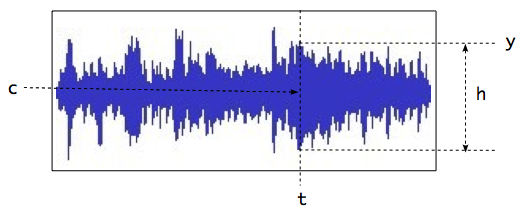
\includegraphics[width=90mm]{imgs/graph}
 \caption{A simple graphic signal, defined at time t by a coordinate y, a thickness h and a color c}
 \label{graphimg}
\end{figure}

%-------------------------------
%:   The signal virtual address space.
\sublevel{The \textit{signal} virtual address space.}
A \OSC{scene} includes a virtual address space, which OSC address is \OSC{/ITL/scene/signal}. This address space is reserved for \emph{simple signals} as well as for composing signals in parallel.

The \OSC{signal} virtual address space supports only the \OSC{get} messages that gives the list of the defined signals with a set of messages complying to the syntax defined in section \ref{ssignal}.

%\begin{rail}
%signal : 'garbage'
%		| 'get'
%\end{rail}
%%		| 'debug' int32
%%		| 'get' (| 'debug')
%\index{signal}
%\index{signal!get}
%\index{signal!garbage}
%%\index{signal!debug}
%
%\begin{itemize}
%\item the \OSC{garbage} message deletes all the \emph{unused} signals i.e. all the signal not connected to a \emph{graphic} signal (see section \fullref{gsignal}. 
%%\item the \OSC{debug} message followed by \OSC{[0,1]} control debug messages sent when xruns are detected.
%\item the \OSC{get} message gives the list of the defined signals with a set of messages complying to the syntax defined in section \ref{ssignal}. 
%%\item the \OSC{get debug} message gives the debug state. 
%\end{itemize}


\subsublevel{Simple signals.}
\label{ssignal}
The signal messages can be sent to any address with the form \OSC{/ITL/scene/signal/\textit{identifier}}, where \OSC{\textit{identifier}} is a unique signal identifier.
The set of messages supported by a signal is the following:
\begin{rail}
simpleSignal : [1] ( float32 + )
		| [2] ('size' int32) 
		| [3] ('default' float32)
		| [4] 'get' ( | 'size' | 'default')
		| [5] 'reset'
		| [6] 'del'
\end{rail}
\index{signal}
\index{signal!simple signal!size}
\index{signal!simple signal!default}
\index{signal!simple signal!get}
\index{signal!simple signal!reset}
\index{signal!simple signal!del}

\begin{itemize}
\item \textbf{[1]} push an arbitrary data count into the signal buffer. The data range should be \values{[-1,1]}. Note that the signal buffer behaves like a ring buffer, thus data are wrapped when the data count if greater than the signal size. 
\item \textbf{[2]} the \OSC{size} message sets the signal buffer size. When not specified, the buffer size value is the size of the first data message. 
\item \textbf{[3]} the \OSC{default} message sets the \emph{default signal value}. A signal \emph{default value} is the value returned when a query asks for data past the available values.
\item \textbf{[4]} the \OSC{get} gives the signal values. The \OSC{size} and  \OSC{default} parameters are used to query the signal size and default values.
\item \textbf{[5]} the \OSC{reset} message clears the signal data. 
\item \textbf{[6]} the \OSC{del} message deletes the signal from the \OSC{signal} space. Note that it is safe to delete a signal even when used by a graphic signal. 
\end{itemize}

\example
\sample{/ITL/scene/signal/null 0.0;}
creates a constant signal named \OSC{null}, which value is \values{0}.

%-------------------------------
%:   Composing signals in parallel.
\subsublevel{Composing signals in parallel.}\label{parcomp}
Composing signals in parallel produces a signal which value at a time \values{t} is a vector of the composed signals values. Thus an additional property is defined on \emph{parallel signals} : the signal \emph{dimension} which is size of the signals values vector. Note that the dimension property holds also for simple signals.
The format of the messages for parallel signals is the following:
\begin{rail}
parallelSignal :  
		  [1] 'set' ( signal + )
		| [2] (| projectionString) ( float32 + )
		| [3] ('get' 'dimension') 
\end{rail}
\index{signal!parallel signal}
\index{signal!parallel signal!get}
where 
\begin{rail}
signal :  
		  [4] identifier
		| [5] float32
\end{rail}
\index{signal!parallel signal!list}

\begin{itemize}
\item \textbf{[1]} defines a new signal composed of the signals list and which address is the message OSC address. A signal list element is defined as:

\begin{itemize}
\item \textbf{[4]} an \OSC{identifier} i.e. a signal name refering to an existing signal in the \OSC{signal} virtual address space. 
\item \textbf{[5]} or as a float value. This form is equivalent to an anonymous constant signal holding the given value. 
\end{itemize}

\item \textbf{[2]} sets the values of the signals addressed by a projection string. See section \fullref{sigproj}. 
\item \textbf{[3]} in addition to the \OSC{get} format defined for signals, a parallel signal supports the \OSC{get dimension} message, which gives the number of simple signals in parallel. It is actually the sum of each signal dimension. The dimension of a simple signal is 1. 
\end{itemize}

Note that for a parallel signal:
\begin{itemize}
\item the \OSC{get} message gives the list of the signals in parallel with the exact form of the composing message in [1]. 
\item the \OSC{get size} message gives the maximum of the components size. 
\item the \OSC{get default} message gives the default value of the first signal. 
\end{itemize}

%-------------------------------
%:   Signals projection.
\subsublevel{Signals projection.}
\label{sigproj}
Individual components of a parallel signal may be addressed using a \emph{projection string} which is defined as:
\begin{rail}
projectionString :  '[' int32 (| '\~{}' (| int32)) ']'
\end{rail}
\index{signal!parallel signal!projection string}

The projection string is made of a \emph{index value}, followed by an optional \emph{parallel marker} (\OSC{\~{}}), followed by an optional \emph{step value}, all enclosed in brackets.
The \emph{index value} \values{n} is the index of a target signal. When the \emph{parallel marker} option is not present, the values are directed to the target signal and the message is equivalent to:
\oldexample \texttt{/ITL/scene/signal/target values...} \\
where \OSC{\textit{target}} is the name of the target signal addressed by \values{n}. \\
Note that:
\begin{itemize}
\item the message is ignored when \values{n} is greater than the number of signals in parallel. Default \values{n} value is \values{0}. 
\item setting directly the values of a simple signal or as the projection of a parallel signal are equivalent.
\end{itemize}

The \emph{parallel marker} (\OSC{\~{}}) and the \emph{step value} \values{w} options affect the target signals. Let's consider \values{s[n]} as the signal at index \values{n}. The values are distributed in sequence and in loop to the signals \values{s[n], s[n+w]...s[m]} where \values{m} is the greatest value of the index \values{n+(w.i)} that is less than the signal dimension. The default  \emph{step value} is \values{1}.

\example \\
the message: 
\sample{/ITL/scene/signal/target [2\~{}] 0.1 0.2}
is equivalent to the following messages:
\ \sample{
/ITL/scene/signal/target [2] 0.1\\
/ITL/scene/signal/target [3] 0.2
}


%-------------------------------
%:   Graphic signals.
\sublevel{Graphic signals.}
\label{gsignal}

A graphic signal is created in the standard scene address space. A simple graphic signal is defined by a parallel signal controling the \values{y} value, the graphic thickness and the color at each time position. The color is encoded as HSBA colors (Hue, Saturation, Brightness, Transparency). The mapping of a signal value  (\values{[-1,1]}) to the HSBA color space is given by the table \ref{hsbamap}. 

\begin{figure}[h]
	\centering 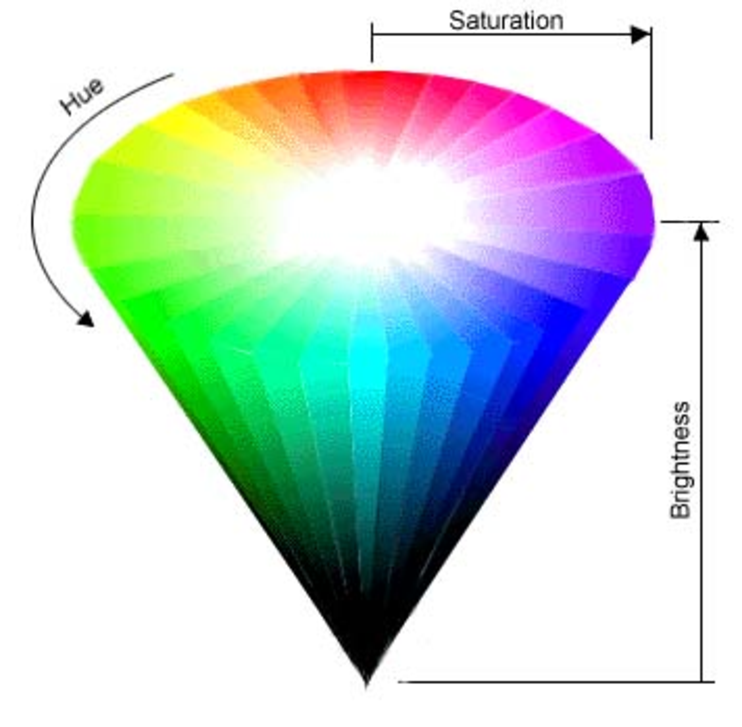
\includegraphics[width=65mm]{imgs/hsb}
 \caption{The HSB color space}
 \label{hsbfiug}
\end{figure}


\begin{table}[htdp]
\caption{HSBA color values.}
\begin{center}
\begin{tabular}{|r|cl|}
\hline
parameter & mapping & \\
\hline
\OSC{hue}				& \OSC{[-1,1]} & corresponds to \OSC{[-180,180]} angular degree where \OSC{0} is red. \\
\OSC{saturation}		& \OSC{[-1,1]} & corresponds \OSC{0\%} to \OSC{100\%} saturation. \\
\OSC{brigthness}		& \OSC{[-1,1]} & corresponds \OSC{0\%} (black) to \OSC{100\%} (white) brithgness. \\
\OSC{transparency}		& \OSC{[-1,1]} & corresponds \OSC{0\%} to \OSC{100\%} tranparency. \\
\hline
\end{tabular}
\end{center}
\label{hsbamap}
\end{table}



A graphic signal responds to common component messages (section \fullref{common}). In addition, it supports the following messages:
\begin{rail}
graphicSignal : 'set' 'graph' signalIdentifier 
			| 'get'
			| 'get' 'dimension'
\end{rail}
\index{Graphic signal!set}
\index{Graphic signal!get}
\index{Graphic signal! dimension}

\begin{itemize}
\item the \OSC{set} message is followed by the \OSC{graph} type and a \OSC{\textit{signalIdentifier}}, where \OSC{signalIdentifier} must correspond to an existing signal from the \OSC{signal} address space. In case \OSC{signalIdentifier} doesn't exist, then a new signal is created at the \OSC{signalIdentifier} address with default values. 
\item the \OSC{get} message is the counterpart of the \OSC{set} message (see section \fullref{getsect}). 
\item the \OSC{get dimension} message gives the number of graphic signals in parallel (see section \fullref{pgsignal}). 
 \end{itemize}

%-------------------------------
%:   Graphic signal default values.
\subsublevel{Graphic signal default values.}
As mentionned above, a graphic signal expects to be connected to parallel signals having at least an \values{y} component, a graphic thickness component and HSBA components. Thus, from graphic signal viewpoint, the expected dimension of a signal should be equal or greater than 6. In case the \OSC{signalIdentifier} dimension is less than 6, the graphic signal will use the default values defined in table \ref{gsigdefault}.

\begin{table}[htdp]
\caption{Graphic signal default values.}
\begin{center}
\begin{tabular}{|r|cl|}
\hline
parameter & default value & \\
\hline
\OSC{y}					& \OSC{0} & the center line of the graphic \\
\OSC{thickness}		& \OSC{0} & \\
\OSC{hue}				& \OSC{0} & meaningless due to brigthness value \\
\OSC{saturation}		& \OSC{0} & meaningless due to brigthness value \\
\OSC{brigthness}		& \OSC{-1} & black \\
\OSC{transparency}		& \OSC{1} & opaque \\
\hline
\end{tabular}
\end{center}
\label{gsigdefault}
\end{table}

%-------------------------------
%:   Parallel graphic signals.
\subsublevel{Parallel graphic signals.}
\label{pgsignal}
When the dimension \textit{d} of a signal connected to a graphic signal is greater than 6, then the input signal is interpreted like parallel graphic signals. More generally, the dimension \textit{n} of a graphic signal is:
\[
n  \  |\ n \in \mathbb{N}\ \land\ 6.(n-1) < d \leqslant 6.n
\]
where \textit{d} is the dimension of the input signal.

Note than when \textit{d} is not a mutiple of 6, then the last graphic signal makes use of the default values mentionned above.


%===============================
%:FAUST plugins
\toplevel{FAUST plugins}
\label{faust}

FAUST [Functional Audio Stream]\footnote{\url{http://faust.grame.fr}} is a functional programming language specifically designed for real-time signal processing and synthesis. A FAUST/INScore architecture allows to embed FAUST processors in INScore, for the purpose of signals computation. A FAUST/INScore plugin is viewed as a parallel signal and thus it is created in the \OSC{signal} address space. Thus and similarly to signals, a FAUST plugin is associated to OSC addresses in the form \OSC{/ITL/\emph{scene}/signal/\emph{name}} where \OSC{\emph{name}} is a user defined name.

\begin{rail}
faustprocessor : 'set' 'faust' "path"
\end{rail}
\index{faustprocessor!set}
A FAUST processor is created with a \OSC{set} message followed by the \OSC{faust} type, followed by the plugin path name. Thus the \OSC{faust} name is a reserved signal name.


%===============================
%:  Specific messages
\sublevel{Specific messages}
\label{faustmsg}
A FAUST processor is characterized by the numbers of input and output channels and by a set of parameters. Each parameter carries a name defined by the FAUST program. The set of messages supported by a FAUST processor is the set of signals messages extended with the parameters names and with specific query messages. 

\begin{rail}
faustmessage : signalMsgs
			 | [1] 'msg' float32
			 | [2] 'get' ('in' | 'out')
\end{rail}
\index{faustprocessor!in}
\index{faustprocessor!out}
\index{faustprocessor!min}
\index{faustprocessor!max}

\begin{itemize}
\item [1] \OSC{\emph{msg}} is any of the FAUST processor parameters, as defined by the FAUST program.
\item [2] the \OSC{get} message is extended to query the FAUST processor: \OSC{in} and \OSC{out} give the number of input and output channels.
% \OSC{msgs} gives the list of the processor specific messages under the form of separate messages including the message name followed by its default, minimum and maximum values.
\end{itemize}


%===============================
%:  Feeding and composing FAUST processors
\sublevel{Feeding and composing FAUST processors}
\label{composefaust}

A FAUST processor accepts float values as input, which are taken as interleaved data.

From composition viewpoint, a FAUST processor is a parallel signal which dimension is the number of output channels. 
Thus, a FAUST processor can be used like any parallel signal. However, the signal identifier defined in \ref{parcomp} is extended to support adressing single components of parallel signal as follows:
\begin{rail}
signal :  
		  identifier ( | "/" n)
		| float32
\end{rail}
where $n$ selects the signal \#n of a parallel signal. Note that indexes start at 0.


%===============================
%:Events and Interaction
\toplevel{Events and Interaction}
\label{interaction}

Interaction messages are user defined messages associated to events and triggered when these events occur. These messages accept variables as message arguments.

The general form of the message is:

\begin{rail}
interactMsg : (('watch' | 'watch+')  ([1] | what  ( | oscMsg))) 
\end{rail}
\index{Interaction!watch}
\index{Interaction!watch+}

\begin{itemize}
\item \OSC{watch}: clears the messages associated to the event and when specified, associates the new message to the watched event. \OSC{watch} without arguments ([1]) clears all the messages associated to all events.
\item \OSC{watch+}: adds a message to the watched event message list. 
\end{itemize}

The associated OSC message is any valid OSC message (not restricted to the Interlude message set), with an extended address scheme, supporting IP addresses or host names and udp port number to be specified as OSC addresses prefix. The message parameters are any valid OSC type or variables (see section \ref{interactvar}).
\begin{rail} 
oscMsg : (| fullAddress)  OSCAddress ( (parameters | variable) + )
\end{rail}

\begin{rail} 
fullAddress : (IPAddress | hostname) ':' port
\end{rail}


%===============================
%:   Interaction messages
\sublevel{Interaction messages}
\label{interactmsg}

Events currently \emph{watchable} are:
\begin{rail}
what : 'mouseDown' | 'mouseUp' | 'mouseEnter' | 'mouseLeave' | 'mouseMove' | 'doubleClick' 
\end{rail}
\index{Interaction!mouseDown}
\index{Interaction!mouseUp}
\index{Interaction!mouseEnter}
\index{Interaction!mouseLeave}
\index{Interaction!mouseMove}
\index{Interaction!doubleClick}


\example
\sample{
/ITL/scene/myObject watch mouseDown "/ITL/scene/myObject" "show" 0;
}
Request the object \OSC{myObject} to watch \OSC{mouseDown} events and send a message to itself.
\sample{
/ITL/scene/myObject watch mouseDown "host.domain.org:12100/an/address" "start";
}
Request the object \OSC{myObject} to watch \OSC{mouseDown} events and send a "start" message to host.domain.org on udp port 12100 to OSC address /an/address

%===============================
%:   Notification messages
\sublevel{Notification messages}
\label{notifymsg}

Events currently \emph{watchable} are:
\begin{rail}
what : 	'timeEnter' timezone | 'timeLeave' timezone 
		| 'durEnter' timezone | 'durLeave' timezone 
		| 'newElement'
\end{rail}
\index{Interaction!timeEnter}
\index{Interaction!timeLeave}
\index{Interaction!durEnter}
\index{Interaction!durLeave}
\index{Interaction!newElement}

\begin{rail}
timezone : int32 int32 int32 int32
\end{rail}
A time zone is defined by 2 dates expressed as rational values (i.e. with 4 integers).
\index{Interaction! timezone}

\begin{itemize}
\item \OSC{timeEnter}, \OSC{timeLeave} are triggered when an object date is moved to or out of a watched \OSC{timezone},
\item \OSC{durEnter}, \OSC{durLeave} are triggered when an object duration is moved to or out of a watched \OSC{timezone} that should be viewed as a duration range.
\end{itemize}

\example \\
 a cursor that displays a given music page when it enters its time zone.
\samplev{
/ITL/scene/cursor watch 'timeEnter' 10 1 18 1 '/ITL/scene/score' 'set' 'img' 'page2.png';
}



The \OSC{newElement} event is supported at scene level only and triggered when a new element is added to the scene.


%===============================
%:   Message variables
\sublevel{Variables}
\label{interactvar}

Variables denote values computed when an event is triggered. These values are send in place of the variable. A variable name starts with a '\$' sign. Currently, the following variables are supported by mouse events:
\begin{rail} 
variable : (xy | 'absx' | 'absy' | 'sx' | 'sy' | date | 'name' | 'address') 
\end{rail}
\index{Interaction!variable!x}
\index{Interaction!variable!y}
\index{Interaction!variable!absx}
\index{Interaction!variable!absy}
\index{Interaction!variable!sx}
\index{Interaction!variable!sy}
\index{Interaction!variable!date}
\index{Interaction!variable!name}
\index{Interaction!variable!address}

\begin{rail} 
xy : ('x' | 'y') ( | '[low,high]') 
\end{rail}

\begin{itemize}
\item \OSC{\$x} \OSC{\$y}: denotes the mouse pointer position at the time of the event. The values are in the range $[0,1]$ where 1 is the object size in the x or y dimension. The value is computed according to the object origin: it represents the mouse pointer distance from the object x or y origin (see \fullref{origin}). \OSC{\$x} and \OSC{\$y} variables support an optional range in the form \OSC{[low, high]} that transforms the $[0,1]$  values range into the $[low, high]$ range.

\item \OSC{\$absx} \OSC{\$absy}: denotes the mouse pointer absolute position at the time of the event. The values represent a pixel position relative to the top-left point of the target object. Note that this position is unaffected by scale. 
Note also that the values are not clipped to the object dimensions and could exceed its width or height or become negative in case of mouse move events.

\item \OSC{\$sx} \OSC{\$sy}: denotes the mouse pointer position in the scene coordinates space. 

\item \OSC{\$name}, \OSC{\$address}: replaced by the target object name or OSC address. Note that in case of \OSC{newElement} event, the target object is the new element. 
\end{itemize}

\begin{rail} 
date : ('date' | 'rdate') (| ':'  mapname) (| '[n/d]') (| '\%' 'f')

\end{rail}

\begin{itemize}
\item \OSC{\$date}: denotes the object date corresponding to the mouse pointer position at the time of the event. It is optionnaly followed by a colon and the name of the mapping to be used to compute the date. The \OSC{\$date} variable is replaced by its rational value (i.e. two integers values). The optional rational enclosed in brackets may be used to indicate a quantification: the date value is rounded to an integer count of the specified rational value. The optional \OSC{\%f} may be used to get the date delivered as a float value.
\item \OSC{\$rdate}: is similar to \OSC{\$date} but ignores the target current date: the date is relative to the object mapping only.
\end{itemize}

Note that a variable can be used several times in a message, but several \OSC{\$date} variables must always refer to the same mapping.

\vspace{5mm}
\texttt{\textbf{Warning:}} the interaction message set is provided for experiment. It is likely to change in a future version. Ideas, comments, suggestions are welcome for the design of a stable API.

%===============================
%:   Message based variables
\sublevel{Message based variables}
\label{msgvar}

A message based variable is a variable containing an OSC message which will be evaluated at the time of the event. They are supported by all kind of events. Like  the variables above, a message based variable starts with a '\$' sign followed by a valid 'get' message enclosed in parenthesis:
\begin{rail} 
msgVar : '(' oscaddress 'get' (| params) ')'
\end{rail}

The evaluation of a 'get' message produces a message or a list of messages. The message based variable will be replaced by the parameters of the messages resulting from the evaluation of the 'get' message.
Note that all the 'get' messages attached to an event are evaluated at the same time.

\example
\sample{ 
/ITL/s/o1 watch  'mouseDown' '/ITL/s/o1' 'show' \$('/ITL/s/o2' get 'show'); \\
/ITL/s/o1 watch+ 'mouseDown' '/ITL/s/o2' 'show' \$('/ITL/s/o1' get 'show'); \\
/ITL/s/o2 watch  'mouseDown' '/ITL/s/o1' 'show' \$('/ITL/s/o2' get 'show'); \\
/ITL/s/o2 watch+ 'mouseDown' '/ITL/s/o2' 'show' \$('/ITL/s/o1' get 'show')
}
When clicked, the objects \OSC{o1} and \OSC{o2} swap their visibility state.



%===============================
%:   OSC address variables
\sublevel{OSC address variables}
\label{oscvar}
The OSC address parameter of a watch message supports the following variables:
\begin{itemize}
\item \OSC{\$self}: replaced by the object name at the time of the message setting.
\item \OSC{\$scene}: replaced by the scene name at the time of the message setting.
\end{itemize}
Note: the system doesn't check for the consistency of the variables placement.


%===============================
%:   States management
\sublevel{States management}
\label{evtstats}

For a given object, its \emph{interaction state} (i.e. the watched events and the associated messages) can be saved and restored.
\begin{rail} 
stateMsg : 'push' | 'pop'
\end{rail}
\index{Interaction!push}
\index{Interaction!pop}

Actually every object embeds a stack to push and pop interaction states. 
\begin{itemize}
\item \OSC{push}: push the current interaction state on top of the stack.
\item \OSC{pop}: replace the current interaction state with the one poped from the top of the stack.
Note that the effect of a pop message addressed to an empty stack is to clear the current interaction state.
\end{itemize}




%===============================
%:Scripting
\toplevel{Scripting}
\label{scripting}

Since INScore saves its states as text files containing lists of OSC messages, it becomes natural to design INSCore scenes using these messages as a textual scripting language. For a better support of scripting, \emph{variables} have been introduced to provide a better parameters control and programming languages have been embedded to generate messages algorithmically.

%===============================
%:   variables
\sublevel{Variables}\label{scriptvar}

A variable may hold any value supported by the parameter types. \oscstring\ must be enclosed in simple or double quotes. It is declared as follows:
\begin{rail} 
variabledecl : 'ident' '=' ( int32 | float32 | string ) ';'
\end{rail}
\index{Scripting! variable}
A variable may be used in place of any message parameter. A reference to a variable must have the form \OSC{\$ident} where \OSC{ident} is a previously declared variable. 

Note that interaction messages may also use variables with similar reference forms (\$ident). There is however no ambiguity concerning these references: interaction variables are always passed as strings and should be quoted, scripts variables as used without quotes.

\example
\sample{
x=0.5;\\
/ITL/scene/a x \$x;\\
/ITL/scene/b x \$x;
}

%===============================
%:   languages
\sublevel{Languages}\label{scriptlang}

\index{Scripting!javascript}
\index{Scripting!lua}

INScore supports Javascript and Lua as scripting languages. Javascript is embedded by default (using the v8 engine - see \url{http://code.google.com/p/v8/}. You need to recompile INScore to embed the Lua engine (\url{http://www.lua.org/}). 

The principle of scripting using a programming language is the following: you can embed \emph{javascript} of \emph{lua} code in an INScore file in a way similar to scripts embedded into html files. This code is expected to produce INScore messages on output.
\begin{rail} 
lang : '<?' ('javascript' | 'lua') script '?>'
\end{rail}
\index{Scripting! language}

The output of the script section is parsed like INScore messages. \\
Note that INScore variables are exported to the current language environment.

\example
\sample{
<?javascript \\
\hspace*{3mm} "/ITL/scene/version set 'txt' 'Javascript v."  + version() + "';"; \\
\hspace*{1mm} ?>
}


A single persistent context is created at application level and for each scene.
It allows scripts to reuse previously defined functions and thus design more structured scripts.

Note: the effect of 'load' message is actually to push the messages on the system stack for
further evaluation. Thus when including a file containing javascript (or lua), the new 
language context won't be available to the next messages in the script. The workaround 
for structured script consists in designing a top level script that only contains 'load' messages.

\example
\sample{
\hspace*{-3mm} /ITL load "javascript-code.inscore";\\
/ITL load "call-javascript.inscore";
}



%===============================
%:Appendix
\toplevel{Appendices}
\sublevel{Grammar definition}
\begin{verbatim}
//_______________________________________________
// relaxed simple INScore format specification
//_______________________________________________
start       : expr
            | start expr
            ;

//_______________________________________________
// expression of the script language
//_______________________________________________
expr        : message  ENDEXPR		
            | variabledecl ENDEXPR	
            | script            
            ;

//_______________________________________________
// javascript and lua support
//_______________________________________________
script      : LUASCRIPT            
            | JSCRIPT            
            ;
//_______________________________________________
// messages specification (extends osc spec.)
//_______________________________________________
message	    : address 
            | address params            
            | address watchparams		
            | address watchparams LEFTPAR messagelist RIGHTPAR
            | address watchparams script 
            ;

messagelist : message            		
            | messagelist COMMA message 
            ;

//_______________________________________________
// address specification (extends osc spec.)
address	    : oscaddress            	
            | urlprefix oscaddress		
            ;

oscaddress  : oscpath            		
            | oscaddress oscpath		
            ;

oscpath	     : PATHSEP identifier		
            | PATHSEP WATCH            	
            | PATHSEP VARSTART varname	
            ;

urlprefix   : hostname COLON UINT		
            | IPNUM COLON UINT            
            ;

hostname    : HOSTNAME            		
            | hostname POINT HOSTNAME	
            ;

identifier  : IDENTIFIER		
            | HOSTNAME            
            | REGEXP            
            ;

//_______________________________________________
// parameters definitions
// watchparams need a special case since messages are expected as argument
//_______________________________________________
watchparams : watchmethod		
            | watchmethod params 

params      : param            	
            | variable            
            | params variable	
            | params param		
            ;

watchmethod : WATCH            	
            ;

variable    : VARSTART varname
            | VARSTART LEFTPAR message RIGHTPAR
            ;

param       : number            
            | FLOAT            	
            | identifier		
            | QUOTEDSTRING		
            ;

//_______________________________________________
// variable declaration
variabledecl : varname EQUAL params	
            ;

varname	    : IDENTIFIER            
            | HOSTNAME            	
            ;

//_______________________________________________
// misc
number      : UINT            		
            | INT            		
            ;
\end{verbatim}


\sublevel{Lexical tokens}
\begin{verbatim}
//_______________________________________________
// numbers
//_______________________________________________
INT       a signed integer
UINT      an unsigned integer
FLOAT     a floating point number

//_______________________________________________
// hosts addresses
//_______________________________________________
// allowed character set for host names (see RFC952 and RFC1123)
HOSTNAME       : [-a-zA-Z0-9]+ 
IPNUM          :  {DIGIT}+"."{DIGIT}+"."{DIGIT}+"."{DIGIT}+

//_______________________________________________
// OSC addresses
//_______________________________________________
// allowed characters for identifiers
IDENTIFIER     : [_a-zA-Z][_a-zA-Z0-9]*
REGEXP           see OSC doc for regular expressions
OSCADDRESS

//_______________________________________________
// strings
//_______________________________________________
STRING          : ("/"|(".""."?"/")*)([^ \t\\/?:*><|"';=]+"/"?)+"."[_a-zA-Z0-9]+
                  or quoted strings that can include any character
                  quotes could be single (') or double quotes (")

//_______________________________________________
// scripting
//_______________________________________________
JSCRIPT        : <?javascript any javascript code ?>
VARIABLE       : the name of a name

//_______________________________________________
// misc.
//_______________________________________________
POINT          : '.'
VARSTART       : '$'
COLON          : ':'
COMMA          : ','
LEFTPAR        : '('
RIGHTPAR       : ')'
EQUAL          : '='
ENDEXPR        : ';'
ENDSCRIPT      : "__END__"
EVAL           : "eval"

//_______________________________________________
// score expressions
//_______________________________________________
EXPRESSION    expr( a valid score expression )
              see 'Score expressions grammar'

//_______________________________________________
// math expressions
//_______________________________________________
ADD            : '+'
DIV            : '/'
EQ             : '=='
GREATER        : '>'
GREATEREQ      : '>='
LESS           : '<'
LESSEQ         : '<='
MINUS          : '-'
MODULO         : '%'
MULT           : '*'
NEG            : '!'
QUEST          : ' ? '
SUB            : '- '
MAX            : '@max' 
MIN            : '@min'

VARIABLEPOSTDEC : $VAR--
VARIABLEPOSTINC : $VAR++
VARIABLEPREDEC  : --$VAR
VARIABLEPREINC  : ++$VAR

\end{verbatim}




%===============================
%:Changes list
\toplevel{ Changes list}


%===============================
%:   Differences to version 0.98
\sublevel{Differences to version 0.98}
\begin{itemize}
\item new \OSC{rate} message at application level to control the time task rate (see section \fullref{ITL})
\item new \OSC{frameless} message at scene level to switch to frameless or normal window (see section \fullref{scene})
\end{itemize}

%===============================
%:   Differences to version 0.97
\sublevel{Differences to version 0.97}
\begin{itemize}
\item new \OSC{fastgraph} object for graphic signals fast rendering (see section \fullref{setsect})
\item \$date variable overflow catched
\item files dropped on application icon correctly opened when the application is not running
\item supports drag and drop of textual osc message strings
\item osc error stream normalized: the message address is 'error:' or 'warning:'
   followed by a single message string.
\item javascript and lua support: a single persistent context is created at application level and for each scene. 
(see section \fullref{scriptlang})
\end{itemize}

%===============================
%:   Differences to version 0.96
\sublevel{Differences to version 0.96}
\begin{itemize}
\item  objects position, date and watched events preserved through type change
\item  bug in quantified dates corrected (null denominator set to the quantified value)
\item  new 'alias' message providing arbitrary OSC addresses support
\item  bug in parser corrected: $backslash$ escape only ' and " chars, otherwise it is literal
\item  guido score map makes use of the new guidolib extended mapping API for staff and system
\item  chords map correction (corrected by guido engine) 
\end{itemize}

%===============================
%:   Differences to version 0.95
\sublevel{Differences to version 0.95}
\begin{itemize}
\item switch to v8 javascript engine
\item lua not embedded by default
\end{itemize}

%===============================
%:   Differences to version 0.92
\sublevel{Differences to version 0.92}
\begin{itemize}
\item new 'mouse' 'show/hide' message supported at application level (see section \fullref{ITL})
\item graphic signal supports alpha messages at object level
\item javascript and lua embedded and supported in inscore scripts  (see section \fullref{scriptlang}).
\item bug correction in sync delete (introduced with version 0.90)
\end{itemize}

%===============================
%:   Differences to version 0.91
\sublevel{Differences to version 0.91}
\begin{itemize}
\item bug corrected: crash with messages addressed to a signal without argument
\item date and duration messages support one arg form using 1 as implicit denominator value 
  the one arg form accepts float values  (see section \fullref{time}).
\end{itemize}

%===============================
%:   Differences to version 0.90
\sublevel{Differences to version 0.90}
\begin{itemize}
\item bug in sync management corrected (introduced with the new sync parsing scheme)
\end{itemize}

%===============================
%:   Differences to version 0.82
\sublevel{Differences to version 0.82}
\begin{itemize}
\item at application level: osc debug is now 'on' by default
\item new scripting features (variables)  (see section \fullref{scriptvar}).
\item ITL file format change: \\
  - semicolon added at the end of each message \\
  - '//' comment not supported any more \\
  - '\%' comment char replaced by '!' \\
  - new variables scripting features \\
  - single quote support for strings \\
  - messages addressed to sync node must use the string format
\item new 'grid' object for automatic segmentation and mapping
\end{itemize}

%===============================
%:   Differences to version 0.81
\sublevel{Differences to version 0.81}
\begin{itemize}
\item new Faust plugins for signals processing
\item colors management change: all the color models (RGBA and HSBA) accept now
  float values that are interpreted in the common [-1,1] range. For the
  hue value, 0 always corresponds to 'red' whatever the scale used.
\item stretch adjustment for video objects (corrects gaps in sync h mode)
\item support for opening inscore files on the command line
\item system mapping correction
\item splash screen and about menu implemented by the viewer
\end{itemize}

%===============================
%:   Differences to version 0.80
\sublevel{Differences to version 0.80}
\begin{itemize}
\item behavior change with synchronization without stretch: now the system looks also in the
  slave map for a segment corresponding to the master date.
\item \OSC{\$date} variable change: the value is now (0,0) when no date is available and \OSC{\$date} is time shifted according to the object date.
\item \OSC{date} message change: the date 0 0 is ignored
\end{itemize}


%===============================
%:   Differences to version 0.79
\sublevel{Differences to version 0.79}
\begin{itemize}
\item corrects the map not saved by the \OSC{save} message issue
\item corrects \OSC{get map} output: 2D segments were not correctly converted to string
\end{itemize}

%===============================
%:   Differences to version 0.78
\sublevel{Differences to version 0.78}
\begin{itemize}
\item crash bug corrected for the 'save' message addressed to '/ITL'
\item message policy change: relaxed numeric parameters policy (float are accepted for int and int for float)
\item bug in \OSC{get watch} for time events corrected (incorrect reply)
\end{itemize}
Known issues:
\begin{itemize}
\item map not saved by the \OSC{save} message 
\end{itemize}

%===============================
%:   Differences to version 0.77
\sublevel{Differences to version 0.77}
\begin{itemize}
\item guido system map extended: supports flat map or subdivided map (see section \fullref{guidomaps}).
\item new \OSC{shear} and \OSC{rotate} transformations messages (see section \fullref{transform}).
\item new \OSC{rename} message to change an object name (and thus its OSC address) (see section \fullref{common}).
\item relaxed bool parameter policy: objects accept float values for bool parameters 
\item automatic numbering of exports when destination file is not completely specified 
  i.e. no name, no extension. (see section \fullref{common}).
\item quantification introduced to \$date variable (see section \fullref{interactvar}).
\item \OSC{reset} message addressed to a scene clears the scene rootPath
\end{itemize}

%===============================
%:   Differences to version 0.76
\sublevel{Differences to version 0.76}
\begin{itemize}
\item  get \OSC{guido-version} and \OSC{musicxml-version} messages supported by the application (see section \fullref{ITL}).
\item  \OSC{save} message bug correction - introduced with version 0.70: only partial state of objects was saved
\item  \OSC{rootPath} message introduced at scene level (see section \fullref{scene}).
\item  scene name translation strategy change: only the explicit 'scene' name is 
  translated by the scene load message handler into the current scene name, 
  other names are left unchanged.
\item  bitmap copy adjustment in sync stretched mode is now only made for images
\end{itemize}


%===============================
%:   Differences to version 0.75
\sublevel{Differences to version 0.75}
\begin{itemize}
\item new \OSC{require} message supported by the \OSC{/ITL} node (see section \fullref{ITL}).
\item new event named \OSC{newElement} supported at scene level (see section \fullref{notifymsg}).
\item new \OSC{name} and \OSC{address} variables (see section \fullref{interactvar}).
\item new system map computation making use of the new slices map provided by the guidolib version 1.42
\item INScore API: the \OSC{newMessage} method sets now the message src IP to localhost
  With the previous version and the lack of src IP, replies to queries or error 
  messages could be sent to undefined addresses (and mostly lost).
\item bug corrected with ellipse and rect : integer graphic size computation changed 
  to float (prevents objects disappearance with small width or height)
\item bug in scene export: left and right borders could be cut, depending  on the scene size
  corrected by rendering the QGraphicsView container instead the QGraphicsScene
\item crash bug with \$date:name corrected: crashed when there is no mapping named \OSC{name}.
\end{itemize}

%===============================
%:   Differences to version 0.74
\sublevel{Differences to version 0.74}
\begin{itemize}
\item new \OSC{map+} message  (see section \fullref{mapAddMsg}).
\item the \OSC{click} and \OSC{select} messages are deprecated (but still supported). They will be removed in a future version (see section \fullref{csmsg}).
\end{itemize}

%===============================
%:   Differences to version 0.63
\sublevel{Differences to version 0.63}
\begin{itemize}
\item new \OSC{dpage} message accepted by \OSC{gmn} objects (see section \fullref{gmnpage}).
\item x and y variables: automatic range type detection (int | float)
\item set \OSC{txt} message: accepts polymorphic stream like parameters (see section \fullref{setsect}).
\item drag and drop files support in INScore viewer
\item interaction variables extension: \OSC{\$sx}, \OSC{\$sy} variables added to support scene coordinate space (see section \fullref{interactvar}).
\item automatic range mapping for \OSC{\$x}, \OSC{\$y} variables.
\item new \OSC{\$self} and \OSC{\$scene} variables in the address field (see section \fullref{oscvar}).
\item OSC identifiers characters set extended with '\_' and '-' (see section \fullref{genformat}).
\item support for multiple scenes: \OSC{new}, \OSC{del} and \OSC{foreground} messages (see section \fullref{scene}).
\item \OSC{load} message supported at scene level (see section \fullref{scene}).
\item \OSC{get watch} implemented.
\item \OSC{watch} message without argument to clear all the watched events (see section \fullref{interactvar}).
\item order of rendering and width, height update corrected (may lead to incorrect rendering)
\item bug with gmn score corrected: missing update for page, columns and rows changes.
\item package delivered with the Guido Engine version 1.41 that corrects minimum staves distance and incorrect mapping when optimum page fill is off.
\end{itemize}

%===============================
%:   Differences to version 0.60
\sublevel{Differences to version 0.60}
\begin{itemize}
\item new 'mousemove' event (see section \fullref{interactmsg}).
\item interaction messages accept variables (\$x, \$y, \$date...) (see section \fullref{interactvar}).
\item SVG code and files support (see section \fullref{setfile}).
\item set line message change: the \OSC{x y} form is deprecated, it is replaced by
  the following forms: \\
  \OSC{'xy' x y} (equivalent to the former form) 
  and \OSC{'wa' width angle}   
  (see section \fullref{setsect}).
\item new 'effect' message  (section \fullref{effectmsg}).
\item utf8 support on windows corrected
\item transparency support for stretched synchronized objects corrected
\item multiple application instances supported with dynamic udp port number allocation.
\item command line option with --port portnumber option to set the receive udp port number at startup.
\end{itemize}

%===============================
%:   Differences to version 0.55
\sublevel{Differences to version 0.55}
\begin{itemize}
\item new 'xorigin' and 'yorigin' messages (section \fullref{origin}).
\item new interaction messages set (section \fullref{interaction}).
\item alpha channel handled by images and video
\item bug correction in line creation corrected (false incorrect parameter returned)
\item bug correction in line 'get' message handling
\item memory leak correction (messages not deleted)
\end{itemize}

Known issues: 
\begin{itemize}
\item incorrect graphic rendering when 'sync a b' is changed to 'sync b a' in the same update loop
\item incorrect nested synchronization when master is horizontaly stretched,
\end{itemize}

%===============================
%:   Differences to version 0.53
\sublevel{Differences to version 0.53}
\begin{itemize}
\item ITL parser corrected to support regexp in message string (used by messages addressed to sync node)
\item format of mapping files and strings changed (section \fullref{mapMsg}).
\item format of sync messages extended to include map name (section \fullref{syncmsg}).
\item signal node: 'garbage' message removed
\item new 'reset' message for the scene (/ITL/scene) (section \fullref{scene}).
\item new 'version' message for the application (/ITL) (section \fullref{ITL}).
\item new 'reset' message for signals (section \fullref{ssignal}).
\item bug parsing messages without params corrected
\item slave segmentation used for synchronization
\item new H synchronization mode (preserves slave segmentation)
\item crash bug corrected for load message and missing ITL files
\end{itemize}

%===============================
%:   Differences to version 0.50
\sublevel{Differences to version 0.50}
\begin{itemize}
\item Graphic signal thickness is now symmetrically drawn around y position.
\item ITL file format supports regular expressions in OSC addresses.
\item IP of a message sender is now used for the reply or for error reporting.
\item new \OSC{line} object (section \fullref{setsect}).
\item new \OSC{penStyle} message for vectorial graphics (section \fullref{specificMsg}).
\item new color messages \OSC{red, green, blue, alpha, dcolor, dred, dgreen, dblue} (section \fullref{common} and  \fullref{relpos}).
\item color values for objects are bounded to [0,255]
\item \OSC{get map} message behaves according to new map message (section \fullref{getsect}).
\item \OSC{get width} and  \OSC{get height} is now supported by all objects (section \fullref{getsect}).
\item  bug in signal projection corrected (index 0 rejected)
\item  bug in signals default value delivery corrected
\item  new \OSC{pageCount} message for guido scores
\item  debug nodes modified state propagated to parent node (corrects the debug informations graphic update issue)
\item rational values catch null denominator (to prevents divide by zero exceptions).

\end{itemize}

%===============================
%:   Differences to version 0.42
\sublevel{Differences to version 0.42}

\begin{itemize}
\item \OSC{identifier} specification change (section \fullref{genformat}).
\item new application \OSC{hello} and  \OSC{defaultShow} messages (section \fullref{ITL}).
\item new \OSC{load} and \OSC{save} messages  (sections \fullref{ITL} and  \fullref{common}).
\item \OSC{click} and \OSC{select} messages (section \fullref{csmsg}):
\begin{itemize}
\item \OSC{rightbottom} and \OSC{leftbottom} modes renamed to \OSC{bottomright} and \OSC{bottomleft}
\item new \OSC{center} mode for the \OSC{click} message
\item query mode sent back with the reply both for \OSC{click} and  \OSC{select} messages
\end{itemize}
\item new \OSC{file}, \OSC{html} and  \OSC{htmlf} types for the \OSC{set} message (section \fullref{setsect}).
\item \OSC{get} syntax change for the \OSC{scene} (section \fullref{sceneget}).
\item \OSC{fileWatcher} messages completely redesigned (section \fullref{watch}).
\item mappings can be identified by names (section \fullref{mapMsg}).
\item rect, ellipse, curve, line and polygon object support graphic to relative-time mapping
\item new synchronization modes for Guido scores: voice1, voice2, ... , staff1, staff2, ... , system, page (section \fullref{guidomaps}).
\item Guido mapping manages repeat bars.
\item Graphic signals messages design (section \fullref{gsignal}).
\end{itemize}


\printindex

\end{document}
